\documentclass[
	paper=A4,
	titlepage=true,
	appendixprefix=true,
	headings=appendixwithoutprefixline,
	fontsize=11pt,
	parskip=half
]{scrreprt}

% Document title and author
\title{Exploring 3D Geovisualisation Techniques and their Applications with Large Datasets using HTML5 and WebGL}
\author{Monica Olejniczak}

% Other information
\newcommand{\supervisor}{Shamus Smith}
\newcommand{\degree}{Bachelor of Engineering (Honours) (Software)}
\newcommand{\school}{School of Electrical Engineering and Computer Science}
\newcommand{\university}{University of Newcastle}
\newcommand{\country}{Australia}
\newcommand{\institute}{\school\\\university, \country}

%!TEX root = ../report.tex

\usepackage[left=30mm,top=35mm,right=30mm,bottom=35mm,headheight=30pt]{geometry}

%%% Line spacing
\usepackage{setspace}
\onehalfspacing

%%% Enforce UTF8 encoding
\usepackage[utf8]{inputenc}

%%% Colors
\usepackage[dvipsnames]{xcolor}

%%% Maths
\usepackage{amsmath}

%%% Header and footer
\usepackage{scrlayer-scrpage}
\ohead{SENG4800B - Individual Final Report}
\cfoot{\pagemark}

% http://tex.stackexchange.com/questions/198830/section-title-with-runin-and-koma-class

%%% Abstract
\usepackage{abstract}
\setlength{\absleftindent}{0pt}
\setlength{\absrightindent}{0pt}
\renewcommand{\absnamepos}{flushleft}
\renewcommand{\abstractnamefont}{\normalfont\Large\bfseries}

%%% Sections
% \usepackage{titlesec}
% \setcounter{secnumdepth}{4}

%%% Tables and figures
\usepackage{wrapfig}
\usepackage{caption}
% Set default font size
\usepackage[font=scriptsize]{subcaption}

%%% Tables
\usepackage{booktabs}
\usepackage{tabularx}

% Table vertical spacing
\renewcommand{\arraystretch}{1.5}
% Add caption spacing
\captionsetup[table]{belowskip=10pt}
% \captionsetup[figure]{belowskip=-10pt}
% \captionsetup[subfigure]{belowskip=10pt}

%%% Figures
% Frames around images
\newcommand{\bordercolor}{black!40}
\newcommand{\figureborder}[1]{%
	\setlength{\fboxsep}{0pt}%
	\setlength{\fboxrule}{0.5pt}%
	\color{\bordercolor}%
	\fbox{#1}%
}

%%% Code
%!TEX root = ../report.tex

\usepackage{courier}
% \usepackage[scaled]{beramono}
% \usepackage[T1]{fontenc}
\usepackage{listings}

% Begin at indentation of environment setup
\usepackage{lstautogobble}

% Define code colors
\definecolor{comment}{RGB}{98,151,85}
\definecolor{keyword}{RGB}{203,119,47}
\definecolor{string}{RGB}{47,95,36}

\lstdefinelanguage{JavaScript}{
	sensitive=false,
	keywords={typeof, new, true, false, catch, function, return, null, catch, switch, var, let, if, in, while, do, else, case, break, class, export, boolean, throw, implements, import, this},
	comment=[l]{//},
	morecomment=[s]{/*}{*/},
	morestring=[b]',
	morestring=[b]"
}

\lstdefinelanguage{GLSL}{
	sensitive=true,
	morekeywords=[1]{
		attribute, const, uniform, varying,
		layout, centroid, flat, smooth,
		noperspective, break, continue, do,
		for, while, switch, case, default, if,
		else, in, out, inout, float, int, void,
		bool, true, false, invariant, discard,
		return, mat2, mat3, mat4, mat2x2, mat2x3,
		mat2x4, mat3x2, mat3x3, mat3x4, mat4x2,
		mat4x3, mat4x4, vec2, vec3, vec4, ivec2,
		ivec3, ivec4, bvec2, bvec3, bvec4, uint,
		uvec2, uvec3, uvec4, lowp, mediump, highp,
		precision, sampler1D, sampler2D, sampler3D,
		samplerCube, sampler1DShadow,
		sampler2DShadow, samplerCubeShadow,
		sampler1DArray, sampler2DArray,
		sampler1DArrayShadow, sampler2DArrayShadow,
		isampler1D, isampler2D, isampler3D,
		isamplerCube, isampler1DArray,
		isampler2DArray, usampler1D, usampler2D,
		usampler3D, usamplerCube, usampler1DArray,
		usampler2DArray, sampler2DRect,
		sampler2DRectShadow, isampler2DRect,
		usampler2DRect, samplerBuffer,
		isamplerBuffer, usamplerBuffer, sampler2DMS,
		isampler2DMS, usampler2DMS,
		sampler2DMSArray, isampler2DMSArray,
		usampler2DMSArray, struct},
		morekeywords=[2]{
		radians,degrees,sin,cos,tan,asin,acos,atan,
		atan,sinh,cosh,tanh,asinh,acosh,atanh,pow,
		exp,log,exp2,log2,sqrt,inversesqrt,abs,sign,
		floor,trunc,round,roundEven,ceil,fract,mod,modf,
		min,max,clamp,mix,step,smoothstep,isnan,isinf,
		floatBitsToInt,floatBitsToUint,intBitsToFloat,
		uintBitsToFloat,length,distance,dot,cross,
		normalize,faceforward,reflect,refract,
		matrixCompMult,outerProduct,transpose,
		determinant,inverse,lessThan,lessThanEqual,
		greaterThan,greaterThanEqual,equal,notEqual,
		any,all,not,textureSize,texture,textureProj,
		textureLod,textureOffset,texelFetch,
		texelFetchOffset,textureProjOffset,
		textureLodOffset,textureProjLod,
		textureProjLodOffset,textureGrad,
		textureGradOffset,textureProjGrad,
		textureProjGradOffset,texture1D,texture1DProj,
		texture1DProjLod,texture2D,texture2DProj,
		texture2DLod,texture2DProjLod,texture3D,
		texture3DProj,texture3DLod,texture3DProjLod,
		textureCube,textureCubeLod,shadow1D,shadow2D,
		shadow1DProj,shadow2DProj,shadow1DLod,
		shadow2DLod,shadow1DProjLod,shadow2DProjLod,
		dFdx,dFdy,fwidth,noise1,noise2,noise3,noise4,
		EmitVertex,EndPrimitive},
		morekeywords=[3]{
		gl_VertexID,gl_InstanceID,gl_Position,
		gl_PointSize,gl_ClipDistance,gl_PerVertex,
		gl_Layer,gl_ClipVertex,gl_FragCoord,
		gl_FrontFacing,gl_ClipDistance,gl_FragColor,
		gl_FragData,gl_MaxDrawBuffers,gl_FragDepth,
		gl_PointCoord,gl_PrimitiveID,
		gl_MaxVertexAttribs,gl_MaxVertexUniformComponents,
		gl_MaxVaryingFloats,gl_MaxVaryingComponents,
		gl_MaxVertexOutputComponents,
		gl_MaxGeometryInputComponents,
		gl_MaxGeometryOutputComponents,
		gl_MaxFragmentInputComponents,
		gl_MaxVertexTextureImageUnits,
		gl_MaxCombinedTextureImageUnits,
		gl_MaxTextureImageUnits,
		gl_MaxFragmentUniformComponents,
		gl_MaxDrawBuffers,gl_MaxClipDistances,
		gl_MaxGeometryTextureImageUnits,
		gl_MaxGeometryOutputVertices,
		gl_MaxGeometryOutputVertices,
		gl_MaxGeometryTotalOutputComponents,
		gl_MaxGeometryUniformComponents,
		gl_MaxGeometryVaryingComponents,gl_DepthRange
	},
	morecomment=[l]{//},
	morecomment=[s]{/*}{*/},
	morecomment=[l][keywordstyle4]{\#}
}

% Default code settings
\lstset{
	autogobble,
	breaklines=true,
	language=JavaScript,
	tabsize=4,
	showstringspaces=false,
	basicstyle=\footnotesize\ttfamily,
	commentstyle=\color{comment},
	keywordstyle=\bfseries\color{keyword},
	ndkeywordstyle=\color{darkgray}\bfseries,
	identifierstyle=\color{black},
	stringstyle=\color{string}
}


%%% References
\usepackage[backend=bibtex,style=authoryear]{biblatex}
\addbibresource{references.bib}

% Change font size
\renewcommand*{\bibfont}{\small}

% Add exclude category with a bibentry command
\DeclareBibliographyCategory{exclude}
\newcommand{\bibentry}[1]{
	\addtocategory{exclude}{#1}
	\fullcite{#1}
}

% Continue footnotes after chapters
\usepackage{chngcntr}
\counterwithout{footnote}{chapter}

%%% Appendices
\usepackage[toc,page]{appendix}

%%% Additional

% Links
\usepackage{hyperref}

% Floats
\usepackage{float}

% Todo notes
\usepackage{todonotes}
\presetkeys{todonotes}{inline}{}


\begin{document}

	%!TEX root = report.tex

%!TEX root = report.tex

\begin{titlepage}
\makeatletter

	\vspace*{\fill}

	{
		\setstretch{1}
		\huge{\textbf{\textsf{\@title}}}
		\par
	}

	\vspace{0.25cm}\par
	{
		\setstretch{1.5}
		\textsf{\LARGE\textbf{\@author}} \\
		\large{Supervised by \supervisor}
		\par
	}
	\vspace{0.25cm}\par

	{
		\setstretch{1}
		\Large{A thesis submitted in partial fulfilment of the requirements for the degree of \degree}
		\par
	}

	\vspace{1.5cm}\par

	\begin{center}
		
\includegraphics[height=3cm]{images/title/uon_logo}
		\vspace{0.25cm}\par
		\Large{\institute}
	\end{center}

	\vspace*{\fill}

	\sffamily
	% \textbf{Date:} \today \\
	% \textbf{Word count:} 14, 000
	\vspace{0.25cm}\par
	\begin{tabularx}{\textwidth}{@{}XX@{}}
		\textbf{Date:} \today & \textbf{Word count:} \wordcount \\
		\textbf{Signed:} \dotfill & \textbf{Signed:} \dotfill \\
		\textbf{Student:} \dotfill & \textbf{Supervisor:} \dotfill \\
	\end{tabularx}

\makeatother
\end{titlepage}

%!TEX root = report.tex

\begin{abstract}

	The web has become a prominent medium for developing geovisualisations, the visualisation of geospatial information, by promoting the creation of highly interactive and immersive environments. Additionally the visualisation of geospatial data is particularly important in the field of data analytics, as geovisualisations facilitate data exploration and decision-making processes when combined with human understanding. This thesis has proposed a method for developing interactive 3D geovisualisations using HTML5 and WebGL to promote the analysis of geospatial data. In order to evaluate whether the system is an effective tool for data analysis, it is essential to consider the usability and performance of the geovisualisations across large datasets.

	This thesis has introduced two types of geovisualisations that were developed using a rapid application development methodology. Another visualisation was created, based off the first geovisualisation, which was integrated into the final year group project as a teaching analytics component. These visualisations can be applied to various datasets by preprocessing the data into an object-based JSON format. The system also features navigation interactions, information displays, filtering tools and custom environment configurations which attempt to further the analysis of geospatial data.

	The system was evaluated by conducting a user study and performance analysis. The results of the user study found that the system was overall easy to use and very consistent. However, users did not feel confident using the system and many features in the user interface and navigation controls could be improved to provide a more positive user experience. Similarly, the performance analysis revealed that the application startup time and run-time performance declined significantly as the size of the dataset increased.

	It was concluded that this system forms a good basis for a prototype to be used in data analytics. However, the system needs several improvements toward its usability and performance before it can be considered an effective tool for the analysis of geospatial data. Further work is recommended to make improvements in the system developed, which have been considered in the future work of this thesis.

\end{abstract}


\newpage

\pagenumbering{roman}
\setcounter{page}{1}

\begin{spacing}{1}
	\tableofcontents
	\listoffigures
	\listoftables
\end{spacing}

\newpage

\pagenumbering{arabic}
\setcounter{page}{1}
	
	\chapter{Introduction} {
	\label{ch:introduction}
		%!TEX root = ../report.tex

This introductory chapter defines what Geovisualisation is, then describes the project and its primary goals and deliverables. Following this, the research questions are discussed.

\section{Geovisualisation} {
\label{sec:geovisualisation}

	Geovisualisation is the interactive visualisation of geospatial information, which is closely related to the fields of scientific and information visualisation~\parencite{jiang2005geovisualization}. Geovisualisations are particularly important in data analytics and when working with large datasets, as visualising geospatial information aids data exploration and decision-making processes when combined with human understanding~\parencite{grinstein2002introduction, hendley1995case}. This is due to the addition of the geographical dimension in the visualisation process, which greatly facilitates the identification and interpretation of spatial patterns and relationships in complex data~\parencite{kwan2004geovisualization}.

}

\section{Project definition} {
\label{sec:project_definition}

	This project focuses on developing geovisualisations in a web environment, to ensure the creation of a platform independent system. The visualisations resemble Figure~\ref{fig:heat_map_financial} and Figure~\ref{fig:3d_representations}, as these designs can be applied to several datasets.

	%!TEX root = ../../report.tex

\begin{figure}[H]
    \newcommand{\figurewidth}{0.5\textwidth}
    \newcommand{\figureheight}{5cm}
	\begin{subfigure}[b]{\figurewidth}
        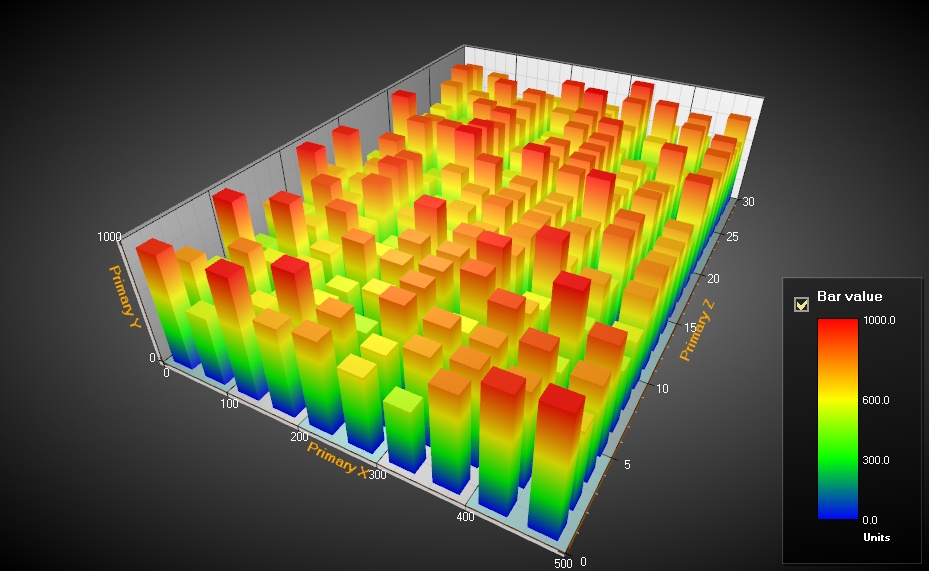
\includegraphics[width=\textwidth,height=\figureheight]{images/introduction/financial}
        \caption{A heat map of financial data. \protect\footnotemark}
        \label{fig:heat_map_financial}
    \end{subfigure}
    \begin{subfigure}[b]{\figurewidth}
        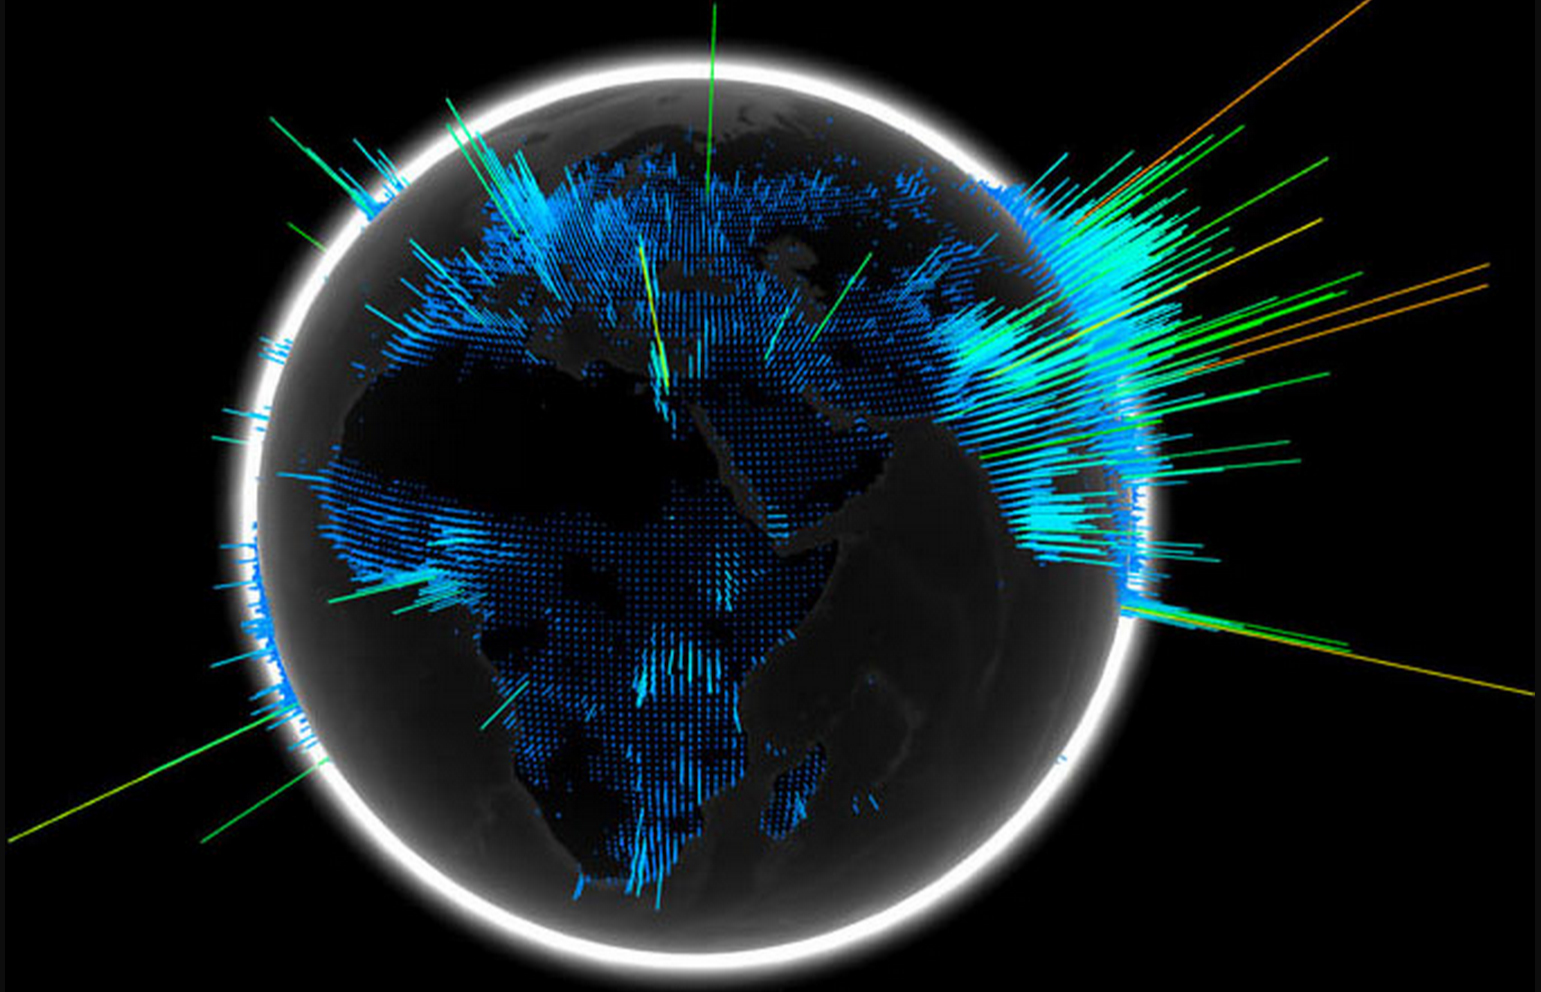
\includegraphics[width=\textwidth,height=\figureheight]{images/introduction/globe}
        \caption{WebGL globe. \protect\footnotemark}
        \label{fig:webgl_globe}
    \end{subfigure}
	\caption[3D representations]{Two different ways of representing 3D data.}
	\label{fig:3d_representations}
\end{figure}

\addtocounter{footnote}{-2}
\stepcounter{footnote}\footnotetext{\bibentry{tuomainen2014financial}}
\stepcounter{footnote}\footnotetext{\bibentry{google2011globe}}


	There is a secondary focus on analysing the performance and scalability between the visualisations, so the system can be designed to cope with large datasets and extended in the future. The primary goals of this project are to:

	\begin{itemize}
		\item Visualise a large dataset in a time efficient manner.
		\item Provide filters to the user and ensure the data can be understood and interpreted without training.
		\item Create visualisations that can be applied to multiple datasets.
		\item Integrate the results into the teaching analytics component of the group project.
		\item Explore how 3D visualisations can effectively convey information.
		\item Apply the visualisations to real datasets and ensure they are scalable.
		\item Explore how to optimise calls and understand what drains processing resources easily.
	\end{itemize}

	The key deliverables of this project have been split into three categories: basic, intermediate and advanced.

	The \emph{basic deliverables} entail developing the implementation for a single visualisation, which should resemble Figure~\ref{fig:heat_map_financial}, with a small, generated dataset. This visualisation will have interactions for panning, zooming and rotating enabling users to navigate the scene.

	The \emph{intermediate deliverables} are concerned with providing users with the ability to filter data, so they are able hide particular information shown on the visualisation. This set of deliverables will also see the implementation of another visualisation, similar to Figure~\ref{fig:heat_map_eeg}, which will initially be applied to a large, generated dataset. The final stage of these deliverables involves applying real datasets, as outlined in Section~\ref{sec:dataset}, to both visualisations.

	The core \emph{advanced deliverables} requires integrating both prototypal visualisations into the group project. Other deliverables include analysing the scalability and computational power to render both visualisations, performing a user study to measure the usefulness of the visualisations and incorporating multi-touch gestures such as pan, pinch, zoom and rotate.
	
}

\section{Research questions} {
\label{sec:research_questions}

	Geovisualisations should effectively display geospatial information in order for a user to establish decision-making processes. Scalability between small and large datasets, network limitations and computer performance must also be considered when a geovisualisation is displayed in a web environment. These concerns result in the following research questions, which will be explored throughout this thesis:

	\begin{itemize}
		\item How can a geovisualisation be visualised in WebGL?
		\item How can a geovisualisation be scaled between small and large datasets?
		\item How can different datasets be applied to 3D geovisualisations?
		\item What is a practical format for a dataset?
		\item Do particular colours have any significant effect on the useability or performance of a geovisualisation?
		\item Do particular filters aid in the analysis of a geovisualisation?
	\end{itemize}

}

	}

	The next chapter will look into the available literature on Geovisualisations.

	\chapter{Related work} {
	\label{ch:related_work}
		%!TEX root = ../report.tex

This chapter explores 3D geovisualisation techniques that could be applied to the project, discusses the World Wide Web as a platform for geovisualisations and common interactions found in 3D geovisualisations. Finally, the applications of geovisualisations are analysed and an overview of the project is provided from this research.

\section{3D geovisualisation techniques} {

	\textcite{bleisch2012geovisualization} defines two distinct categories that represent most 3D geovisualisations: 3D representations of the real world and a combination of 3D representations of the real world with abstract data.

	The \emph{3D representations of the real world} category represents the real world and its objects in realistic or generalised ways to communicate information. This category often uses x, y and z coordinates to show the real world dimensions \textendash\, easting, northing, elevation and sometimes the height of buildings or other objects. A 3D environment attempting to represent the real world usually consists of a digital elevation or surface model with either high resolution orthoimagery, satellite imagery or maps~\parencite{bleisch2012geovisualization}.

	\begin{figure}
	\centering
	\captionsetup{font=small}
    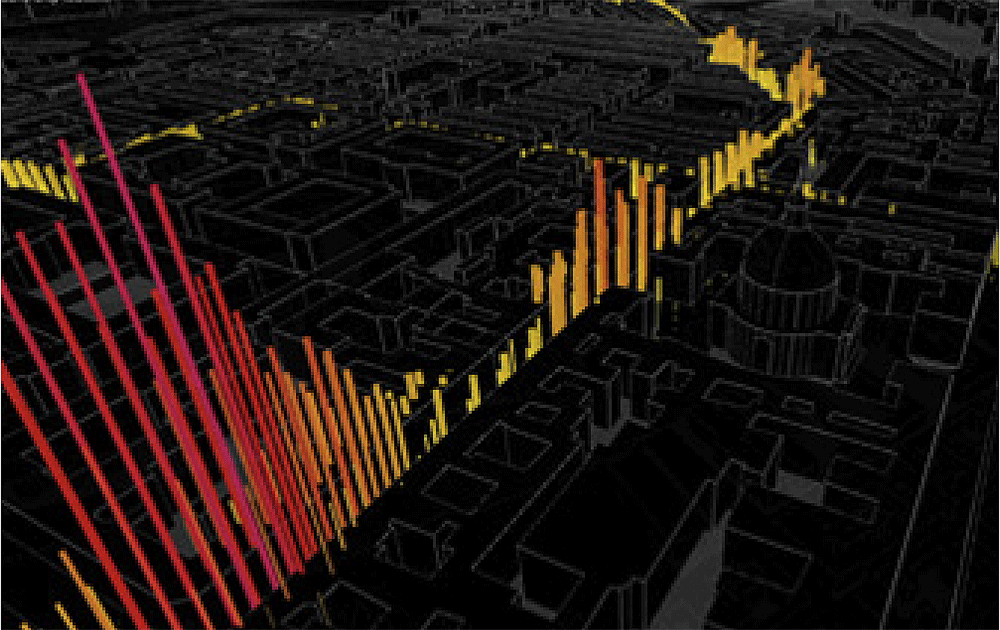
\includegraphics[width=0.8\textwidth]{images/literature/category-combination}
	\caption{An example of combining 3D representations of the real world with abstract data. \protect\footnotemark}
	\label{fig:category_combination}
\end{figure}

\footnotetext{\bibentry{ratti2010copenhagen}}


	Common examples of this category are digital city models and virtual globes. 3D city models often apply photo texturing to suggest additional detail, since the detail may not be present in the underlying geometric model of the city~\parencite{bleisch2012geovisualization}.

	In the \emph{combination of 3D representations of the real world with abstract data} category, the representation of the real world environment is enhanced with the inclusion of data displays. This category aims to communicate, analyse and explore data, where real world dimensions and data values are depicted through the x, y and z axes. An example of this category is shown in Figure~\ref{fig:category_combination} \parencite{bleisch2012geovisualization}.

	To visualise the data displays in this category, triangle based meshes, texture maps or non-uniform rational B-spline surfaces (NURBS) can be created and applied to the visualisation. NURBS in particular are computationally efficient and effective at modelling complex structures~\parencite{hildebrandt2011image, zhong2006enhanced}.

}

\section{Geovisualisations using the World Wide Web} {

	Geovisualisations can be realised through the World Wide Web, which has become a prominent medium for publishing geospatial data. The web facilitates the creation of immersive and highly interactive environments, which can be taken advantage of to explore and present dynamic geospatial data~\parencite{maceachren2001research}.

	WebGL is a cross-platform web standard for a 3D graphics API derived from OpenGL, which has been exposed through the HTML5 canvas element~\parencite{marrin2011webgl} as a drawing context. It is widely supported in modern browsers, without needing additional plug-ins or extensions, and is designed for building dynamic applications that require 3D visualisations~\parencite{chaturvedi2015web, marrin2011webgl, parisi2012webgl}. Rendering such visualisations in real-time is possible due to the accelerated graphics rendering provided by WebGL, which utilises the graphics card memory on a device~\parencite{chaturvedi2015web} to perform multiple operations in parallel to one another.

}

\section{Interaction in geovisualisations} {

	The communication between a user and a system, otherwise known as \emph{interaction}, is an important aspect in geovisualisation. Interaction enables users to explore the data presented to them in order to uncover trends and allow for decision-making processes~\parencite{yi2007toward}. It is also essential for visualisations to support interaction, otherwise the usefulness of the visualisation is greatly limited as the dataset that it represents grows larger~\parencite{yi2007toward}.

	In the context of geovisualisation, the user should be able to navigate the visualisation itself and the synthetic geography that it represents. Navigation enables particular and pertinent information to be located more successfully and is considered to be one of the most important metaphors for dynamic cartography~\parencite{cartwright2001geospatial}. The navigation of a geospatial representation requires the user to perform standard operations, which include: translate, scale, rotate, map projection, manipulation of the design representation parameters, level of generalisation and field of view~\parencite{cartwright2001geospatial, hand1997survey}.

}

\section{Applications of geovisualisation} {

	% equipped assist

	There is a comprehensive amount of geospatial data available, which has been made accessible through various digital data resources. Census enumerations, health statistics, land use categories, meteorological measurements, telephone information and transportation records constitute examples of geospatially referenced data that can be applied to geovisualisations for scientific, research and societal purposes. Furthermore, this widely accessible geospatial data has resulted in an equally large range of application domains for geovisualisations, which include earth science, public health and social science as shown in Figure~\ref{fig:geovisualisation_applications} \parencite{maceachren2004geovisualization}.

	\newcommand{\applicationwidth}{0.32\textwidth}
\newcommand{\applicationheight}{3cm}
\begin{figure}[H]
	\centering
    \begin{subfigure}[b]{\applicationwidth}
        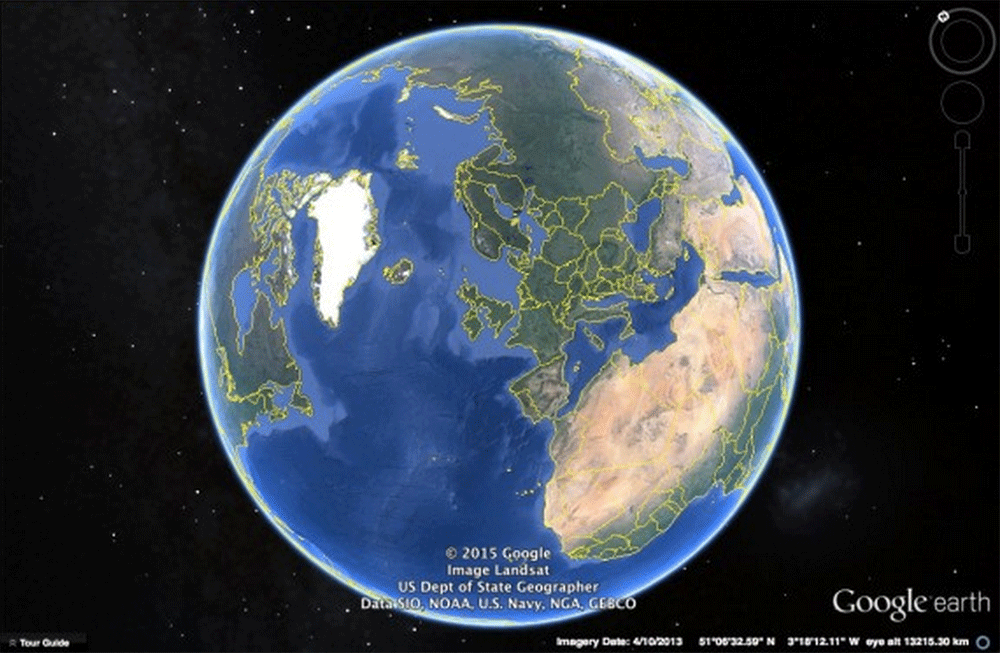
\includegraphics[width=\textwidth,height=\applicationheight]{images/literature/earth-science}
        \caption{Earth science \parencite{google2015earth}}
        % \protect\footnotemark}
        \label{fig:earth_science}
    \end{subfigure}
    \begin{subfigure}[b]{\applicationwidth}
        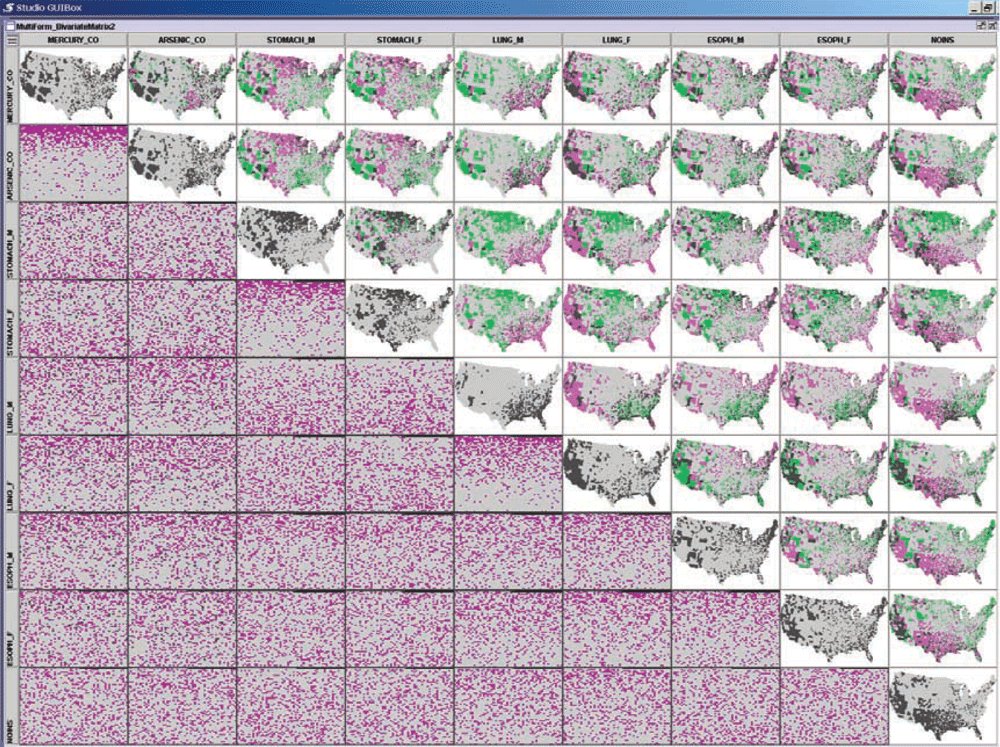
\includegraphics[width=\textwidth,height=\applicationheight]{images/literature/public-health}
        	\caption{\tiny{Public health \parencite{maceachren2004geovisualization}}}
        \label{fig:public_health}
    \end{subfigure}
    \begin{subfigure}[b]{\applicationwidth}
        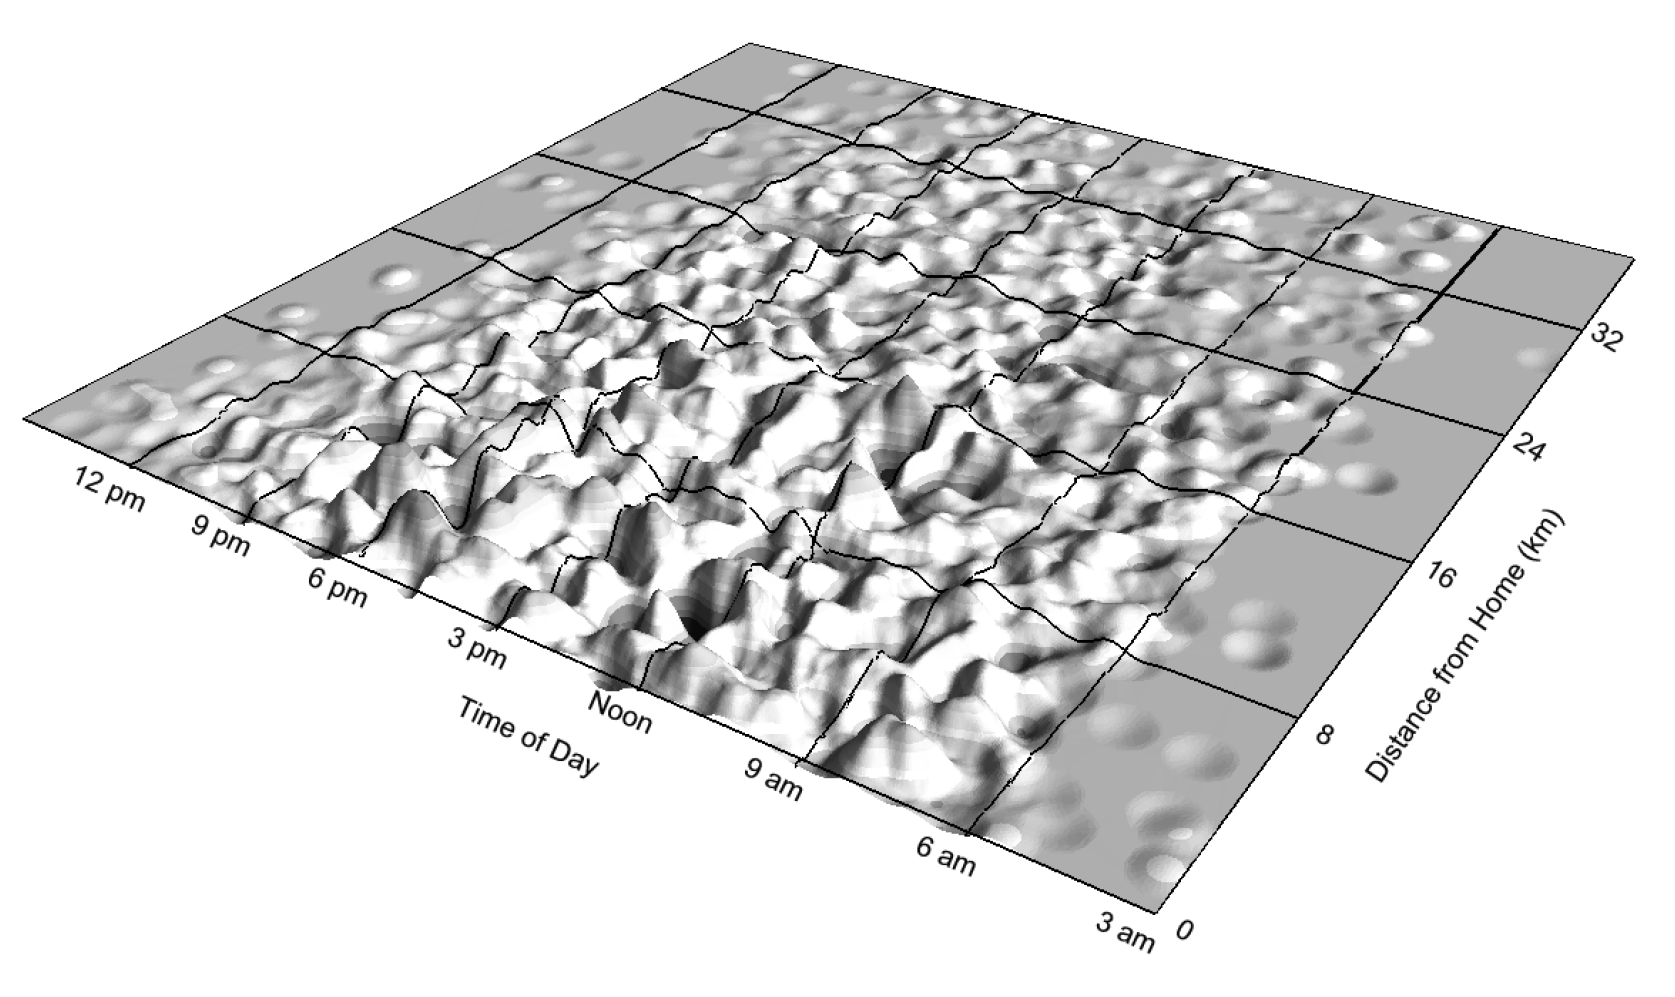
\includegraphics[width=\textwidth,height=\applicationheight]{images/literature/social-science}
        	\caption{Social science \parencite{kwan2004geovisualization}}
        \label{fig:social_science}
    \end{subfigure}
	\caption{Examples of geovisualisations used in various application domains.}
	\subfigcaptionskip
	\label{fig:geovisualisation_applications}
\end{figure}

% \footnotetext{\bibentry{google2015earth}}

	% Earth science
	In the domain of \emph{earth science}, the visualisation of environmental data reveals new insights into the patterns of nature and human-related phenomena. These visualisations also help improve the understanding of the dynamic processes of earth systems~\parencite{yu2012google}.

	\textcite{yu2012google} analyses virtual globes as a tool in earth science applications, which have been developed to effectively facilitate data collection, exploration and the visualisation of environmental data. They deliver huge volumes of satellite imagery, 3D views of the earth, topographic maps and distance measurement to the general public. These globes have promoted entertainment, education, the exploration of new findings, data sharing and provided researchers with effective channels of communicating their findings. Virtual globes can be applied to many areas and in the case of \emph{Google Earth}, typically focus on large-scale phenomena in the atmosphere, carbon science, ecosystems, energy, geology and natural disasters.

	% Public health
	Within \emph{public health}, geovisualisations can be modelled to geospatial data concerning risk factors, health outcomes and interventions to provide an opportunity to understand and act on the varied geographic distribution of disease. However, these datasets are typically difficult to analyse through traditional methods as the data is highly multivariate~\parencite{maceachren2004geovisualization}.

	\textcite{maceachren2004geovisualization} were able to apply a mortality and risk factor dataset to a geovisualisation, in order to explore the spatial and nonspatial relationships in this data. They considered environmental risk factors, health care access and cancer mortality rates of various ages and genders to demonstrate that it is possible to utilise geovisualisations in a way that addresses critical issues in public health.

	% Social science
	An important research area in \emph{social science} is the study of human activities and movements in space and time. Geovisualisations can model this data, which has become feasible with the increased availability of georeferenced individual-level data~\parencite{kwan2004geovisualization}.

	\textcite{kwan2004geovisualization} studied gender and ethnic differences in space-time activity patterns in a metropolitan area. Their study demonstrated that geovisualisation methods are effective in revealing the complex interaction between the spatial and temporal dimensions in structuring human spatial behaviour. \citeauthor{kwan2004geovisualization} also discovered that geovisualisation tools can help formulate more realistic computational or behavioural models for exploratory spatial data analysis.

}

\section{Overview} {

	In this work, HTML5 and WebGL has been used to visualise geographical data, with triangle based mesh data displays. This ensures the development of a cross-platform system capable of rendering complex visualisations through accelerated graphics rendering. This project has considered three navigation interaction techniques: translation, scaling and rotation. Finally, the visualisations have been applied to both a social science dataset due to their wide array of applications and integrated into a live system for teaching analytics.

}

	}

	It has been demonstrated that there are many interesting ways to visualise geographical data with various datasets. To produce a quality system, the design of the project should be considered thoroughly. As such, the next chapter will explore the design of the system and the software methodology utilised throughout the development of this project.
	
	\chapter{Design} {
	\label{ch:design}
		\todo{Purpose of the chapter
 Structure of the chapter
 Central themes of the chapter}

\section{Non-functional requirements} {
\label{sec:non_functiona_requirements}

	The following non-functional requirements are considered key to the success of this project:

	\begin{description}
		\item[Modularity:] The project should be highly modular, so parts of the system can be reused and easily integrated into the group project.
		\item[Performance:] The response time of the system is a major concern when working with a large dataset. The time to load the visualisation is highly dependent on the size of the dataset, graphical processing, network bandwidth and latency. However, once the visualisation has loaded, the user should be faced with near immediate response times (\textless 1 second).
		\item[Scalability:] This is important when modifying the size of the dataset used with a visualisation. The visualisation should be capable of handling increased processing with a larger dataset. Not only this, but the information should remain mapped to the correct locations in the scene with increased volumes of data.
		\item[Testability:] Highly testable code is important when writing test suites, so all aspects of the system can be easily tested to locate faults. In JavaScript:
			\begin{itemize}
				\item A common technique is to hide variables through the use of closure, which leads to untestable code. These variables should be replaced with public variables that are prefixed with an underscore, to indicate they are not a part of the public API.
				\item Promises should not be used within a constructor.
				\item Anonymous functions should be replaced with named functions so they can be tested.
				\item Dependency injection should be used through RequireJS, so all dependencies can be mocked.
			\end{itemize}
	\end{description}

}

\section{Methodology} {
\label{sec:methodology}

	A rapid application development (RAD) approach was undertaken when developing this project. This methodology focuses on iterative development and the rapid construction of prototypes, instead of investing significant amounts of time into planning. RAD enables the software to be written quickly through the reuse of software components and engaging in less formal reviews. This process also performs unit, integration and system testing at the end of each construction phase.

	\todo{insert diagram}

	In this project, each visualisation can be thought of as a single prototype, where parts of the first prototype can be reused for the second visualisation. Testing should be performed during the course of the project, but particularly when a major component of a prototype has been developed, such as data filtering.

	\todo{iterative, agile}

	% An agile methodology will be used throughout the project, as it promotes iterative development, adaptive planning, early prototyping, and encourages flexible and rapid response to changing requirements. This is in contrast to the more traditional methodology, waterfall, which implies a much more rigid workflow, where all requirements are set in stone early in the project. The agile approach gives the project more flexibility, which is required for a project of greater complexity.
	
	% \subsection{Scrum} {

	% 	Scrum is an iterative and incremental agile methodology, in consists of short iterative `sprints' of focused development. The decided sprint length of this project 2 weeks, and conveniently corresponds with the fortnightly client meetings.
		
	% 	Before each sprint, tasks are created and prioritised. These tasks are then assigned evenly across team leaders, and then are further distributed to their team members. This process can take a day or so after the last sprint has finished, using the client's feedback as motivation as to what to include in the sprint. A sprint is then started, and development is generally 'locked' until the completion of the sprint. This keeps teams focused on the issues for the sprint, which have been decided to be the most important.
		
	% 	The chosen issue tracking tool, JIRA, wholly supports the scrum methodology, with in-built features for creating sprints, epics and user stories. This in-built tooling support, combined with its iterative development cycle, makes Scrum a convenient and appropriate methodology for the project.
		
}

\section{Dataset} {
\label{sec:dataset}

	As discussed in Section~\ref{sec:project_definition}, the visualisations began with generated data so development could begin immediately. Using generated data brings control over the size of the dataset applied to a prototype and enables the scalability of each visualisation can be tested. 

	\todo{convert rest of stuff from interim to past tense and make datasets solid}

	% Following the use of fake data, each prototype had real datasets applied to them. By using the same data for both prototypes, their differences in computational requirements and scalability could be compared and analysed. GeoNames~\footnote{\bibentry{wick2005geonames}} is a geographical database that stores population data for a significant number of cities and their respective latitude and longitude coordinates. This database falls under a creative commons attribution license and will be used for both visualisations because there are no copyright concerns or immediate issues when reading and parsing the data it provides. However, some unnecessary information contained in a GeoNames dataset (such as \emph{geonameid}, \emph{feature class} and  \emph{dem}) will need to be removed. The format of the data should also be modified (from a tab separated list to a JavaScript array) when used with a prototype. These steps are necessary so the visualisations can read the data efficiently and hence reduce the loading time for the user. Other datasets can be obtained from Earthdata~\footnote{\bibentry{nasa2000data}}, but will require further investigation regarding how to extract the information from the available databases.

	% Once real data has been applied to both prototypes, the visualisations will be integrated into a live system for the teaching analytics component of the final year project. The amount of touch gestures that particular system components receive and the progress made by students, groups and tutorials will need to be collected and stored in the database. This data can be visualised to aid teachers in analysing ongoing student progress.

	\subsection{Structure} {
	\label{sec:dataset_structure}

		\todo{mention flat vs metadata, performance issues}


	}

}

\section{User interface} {
\label{sec:user_interface}

	The user interface for this system has combined Google's Material Design with a 3D environment, to simplify the way users interact with the system.

	\subsection{Material Design} {
	\label{sec:material_design}

		Material Design is a visual language developed by Google that synthesises classic design principles with current technologies. This design revolves around three principles which have been defined in Figure~\ref{fig:material_design_principles}.

		\newcommand{\materialwidth}{0.328\textwidth}
\begin{figure}[H]
	\centering
	\begin{subfigure}[b]{\materialwidth}
		
\includegraphics[width=\textwidth]{images/design/material/metaphor}
		\caption{Material is the metaphor}
		\label{fig:material_design_metaphor}
	\end{subfigure}
	\begin{subfigure}[b]{\materialwidth}
		
\includegraphics[width=\textwidth]{images/design/material/bold}
		\caption{Bold, graphic, intentional}
		\label{fig:material_design_bold}
	\end{subfigure}
	\begin{subfigure}[b]{\materialwidth}
		
\includegraphics[width=\textwidth]{images/design/material/motion}
		\caption{Motion provides meaning}
		\label{fig:material_design_motion}
	\end{subfigure}
	\caption[Material Design principles]{Material Design principles.}
	\label{fig:material_design_principles}
\end{figure}


		Material Design uses the fundamentals of light, surface and movement to convey how objects move, interact and exist in space and in relation to each other. Elements such as typography, grids, space and colour have been designed to create meaning, maintain user focus and establish a hierarchy using depth effects. These principles aim to provide users with a unified experience across platforms and device sizes, by focusing on user actions and retaining continuity between transitions~\footnote{\bibentry{google2015material}}.

		Material Design details many component specifications that have been implemented by many CSS3 frameworks. Some component examples may be seen in Figure~\ref{fig:material_design_examples}.

		%!TEX root = ../../report.tex

\begin{figure}[H]
	\centering
    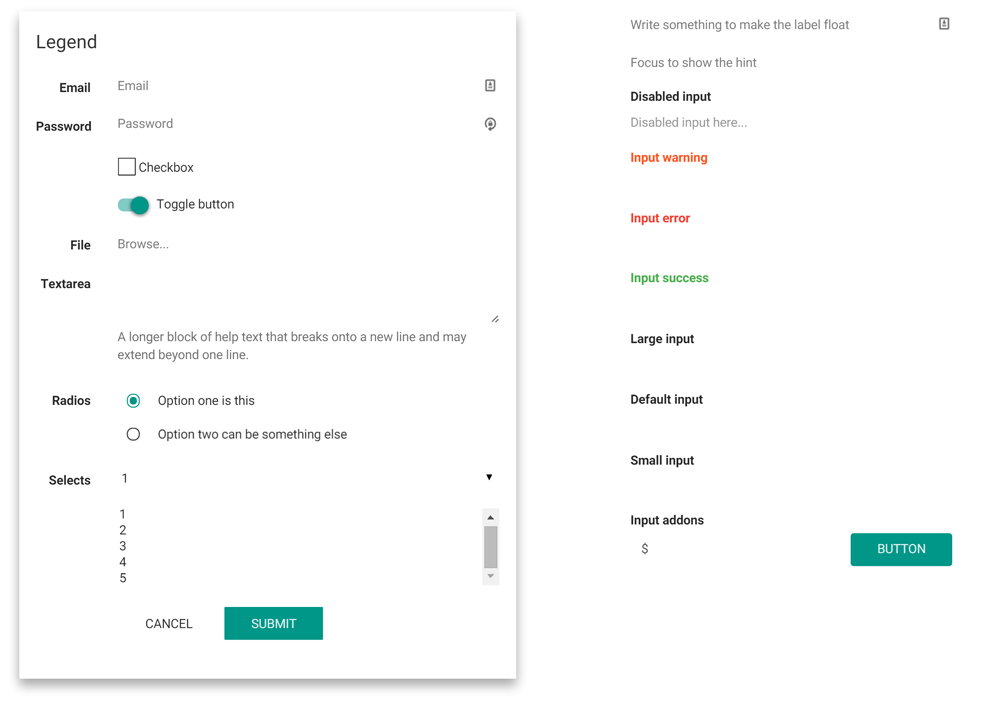
\includegraphics[width=0.7\textwidth]{images/design/bootstrap_material_design}
    \caption[Material Design examples]{Material Design examples\protect\footnotemark.}
    \label{fig:material_design_examples}
\end{figure}

\footnotetext{\bibentry{vrasta2014material}}


		Google Material Design provides an immersive experience to users by adhering to good design principles. Material Design is a great design tool that has been incorporated into the existing infrastructure this project. The group project already makes use of Bootstrap Material Design, a CSS3 framework that adheres to the Google Material Design specifications. As a result of this, a teacher can transition from one system to the other seamlessly, because both systems apply the same design standards.

	}

	\subsection{3D environment} {
	\label{sec:3d_environment}

		The visualisation being viewed by a user features a 3D environment. It has been designed with the following in mind:

		\begin{itemize}
			\item Navigation interactions -- pan, zoom and rotate.
			\item Data points that represent the dataset are displayed as either 3D bars or NURBS.
				\begin{itemize}
					\item Data points should have the ability to be filtered.
				\end{itemize}
			\item The colour of a data point should be effected by the value it represents.
				\begin{itemize}
					\item e.g. Data points that represent population data may be coloured red, orange or yellow to indicate high, medium or low population areas respectively.
				\end{itemize}
			\item Information associated with a data point can be viewed by a user.
				\begin{itemize}
					\item Information is retrieved through metadata. 
					\item Can be shown through hover effects or by outputting the dataset on the page.
				\end{itemize}
			\item Data points are projected from a base geometry.
				\begin{itemize}
					\item The geometry can be a plane or sphere and depends on the dataset being used.
				\end{itemize}
			\item A skybox should serve as a static background for the environment.
		\end{itemize}

		Example mockups of the 3D environment that fulfil the above criteria have been demonstrated in Figure~\ref{fig:environment_mockups}.

		%!TEX root = ../../../report.tex

\begin{figure}[H]
    \newcommand{\figurewidth}{0.5\textwidth}
    \newcommand{\figureheight}{3cm}
	\begin{subfigure}[b]{\figurewidth}
        \centering
        \raisebox{0.5\height}{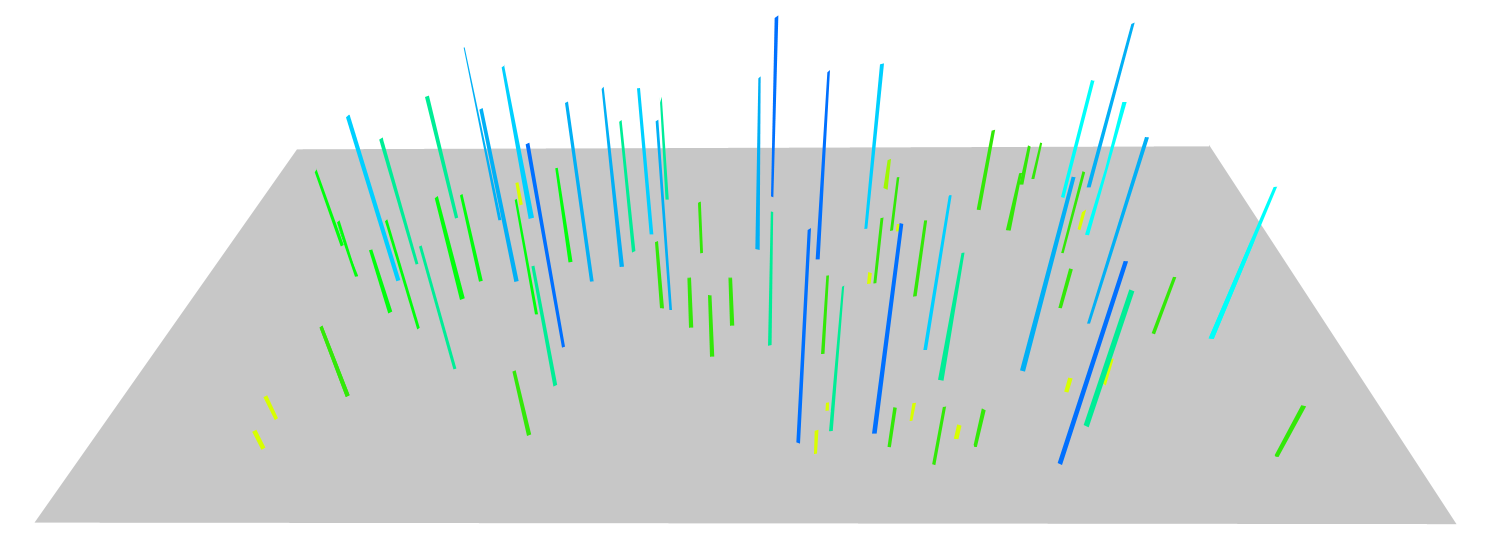
\includegraphics[width=\textwidth]{images/design/mockups/flat}}
        \caption{Visualisation using a flat surface.}
        \label{fig:visualisation_flat}
    \end{subfigure}
    \begin{subfigure}[b]{\figurewidth}
        \centering
        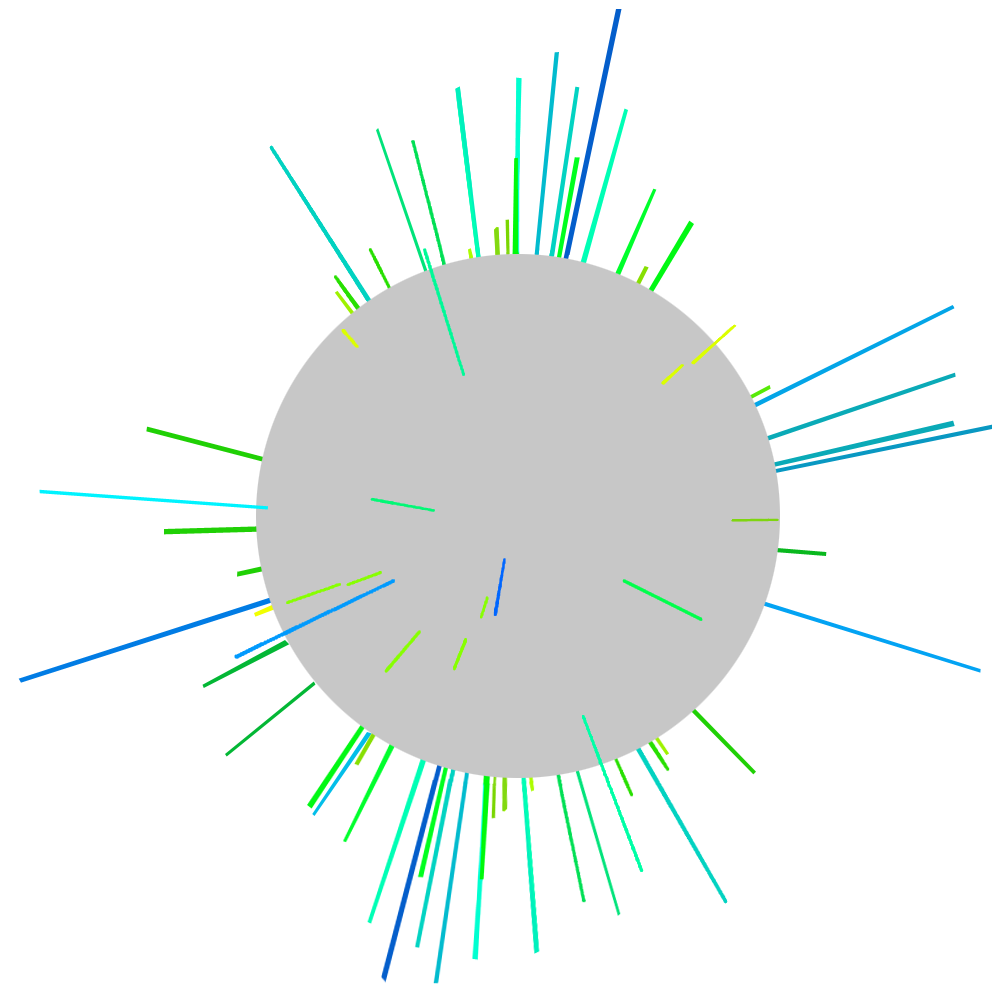
\includegraphics[width=\textwidth]{images/design/mockups/sphere}
        \caption{Visualisation using a sphere surface.}
        \label{fig:visualisation_sphere}
    \end{subfigure}
	\caption[3D environment mockups]{3D environment mockups.}
	\label{fig:environment_mockups}
\end{figure}


	}

	\subsection{Interface design} {
	\label{sec:interface_design}

		The design of the interface needs to account for both the use of Material Design and the 3D environment. 

		Material Design is renowned for its sliding drawer menu, often used to maximise the viewing space for the user. This component has the potential to maintain user focus on the visualisation, while providing additional information through an unobtrusive menu. An initial mockup of this design has been demonstrated in Figure~\ref{fig:user_interface_mockup}, where the 3D environment fills the content to the right of the drawer. This design has been refined through the implementation phase described in Section~\ref{sec:features}.

		\todo{possibly change section reference later}

		%!TEX root = ../../../report.tex

\begin{figure}[H]
	\centering
    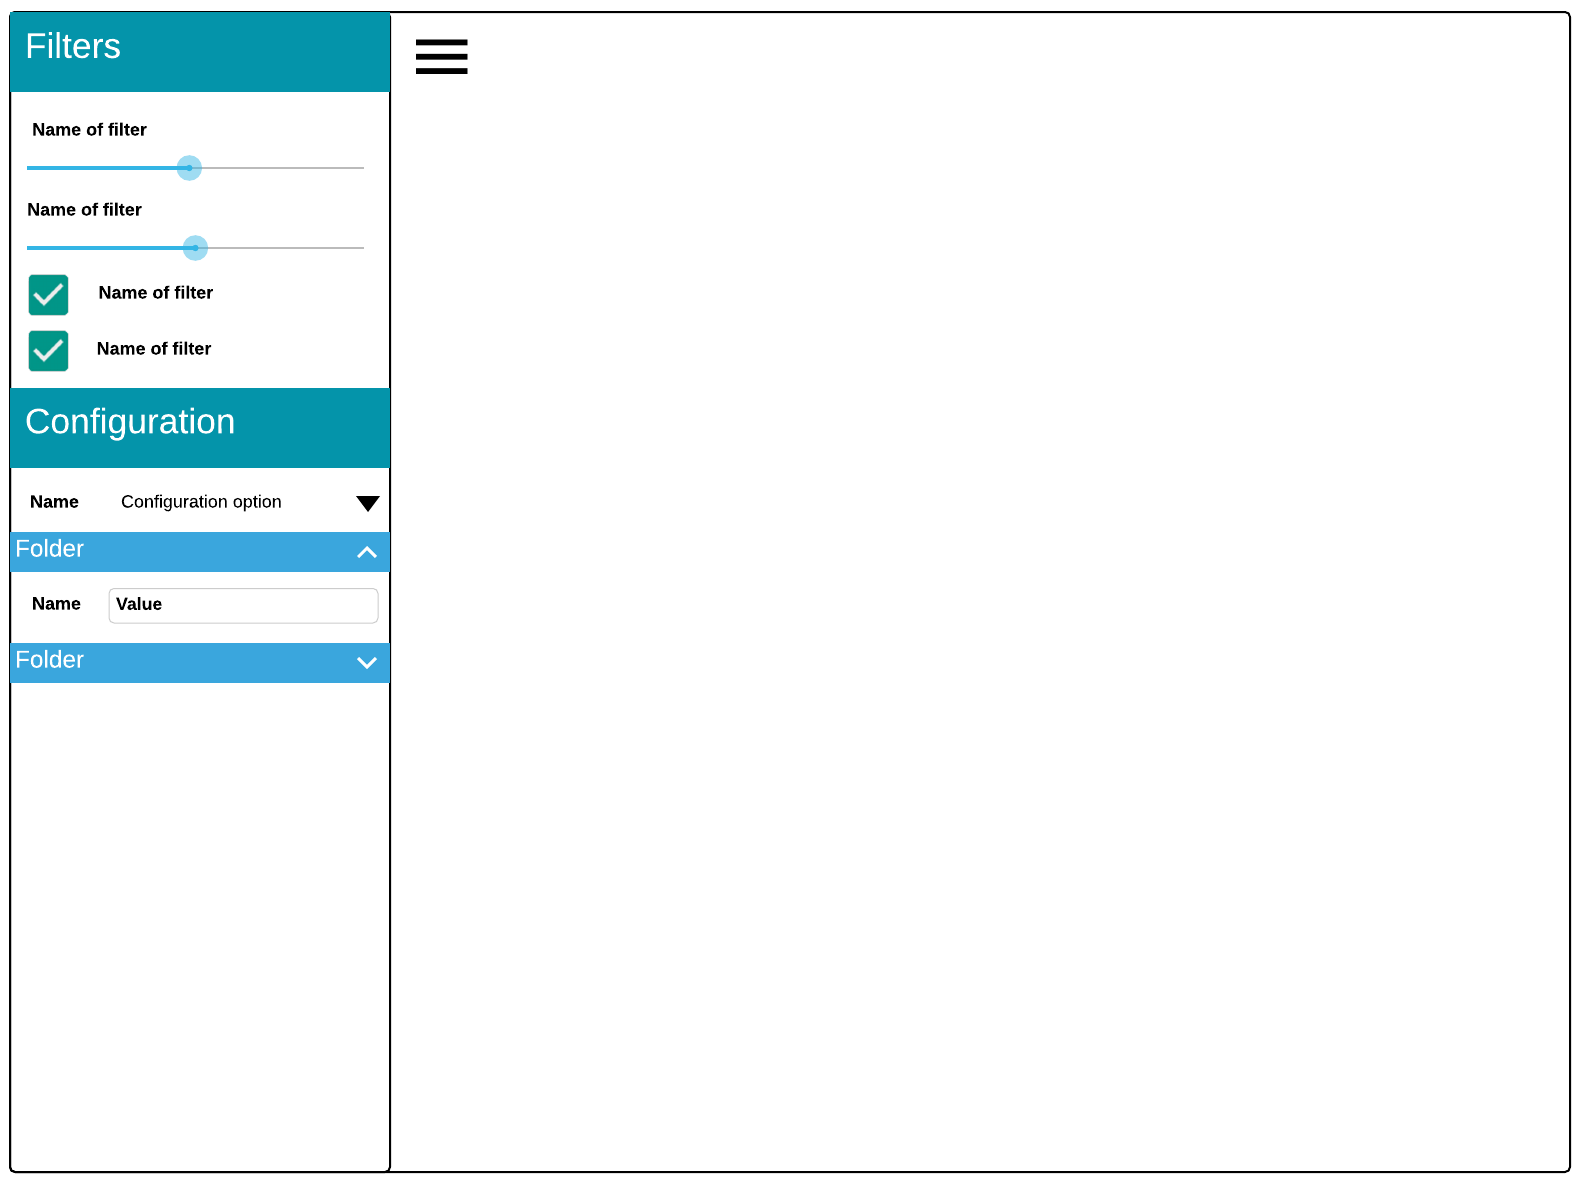
\includegraphics[width=\textwidth]{images/design/mockups/interface}
    \caption[User interface mockup]{User interface mockup.}
    \label{fig:user_interface_mockup}
\end{figure}


		The sliding drawer utilises Material Design components and incorporates two main features -- filtering and live configuration.

		\subsubsection{Filtering} {
		\label{sec:filtering}

			Filters take advantage of slider and checkbox widgets to adjust the state of what is displayed to the user.

			\emph{Sliders} adjust what data points are visible to the user. This is achieved by configuring the bounds of the available metadata in a data point. Take for example a dataset that has a range of values between 0 -- 100. If the user adjusts the value of its respective slider to be $\ge$20, then any data points that have a value \textless20 will be hidden.
			
			\emph{Checkboxes} are designed to be toggled on or off. This widget toggles what metadata associated with a data point is displayed to the user.

		}

		\subsubsection{Configuration} {
		\label{sec:configuration}

			Configuration options are designed to change the values and attributes of the 3D environment in real-time. They are organised in a folder structure, to deliver a hierarchy and logical grouping to the user. Moreover, these options should handle configuring data points and surface values.

			\emph{Data point} configurations should modify the low, medium, high colour values and the range of colours displayed.

			\emph{Surface} configurations should modify the midtone colours of the surface and the colour or intensity of other surface attributes.

		}

	}

}

\section{User actions} {
\label{sec:user_actions}

	The interactions that a user can perform when using this system have been represented in Figure~\ref{fig:user_actions}.

	\todo{not sure if the includes are correct? I'm bad at use-case diagrams :c}

	%!TEX root = ../../report.tex

\begin{figure}[H]
	\centering
    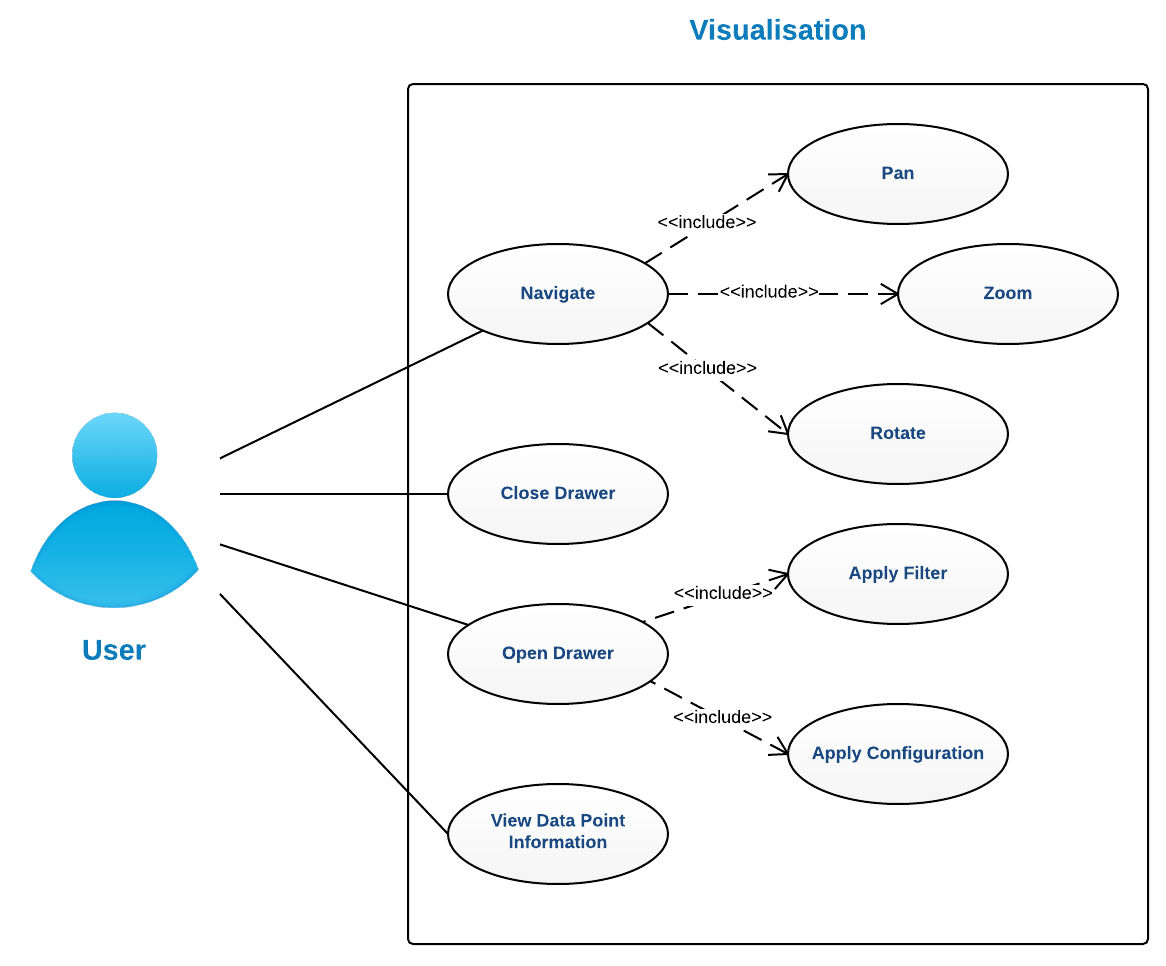
\includegraphics[height=10cm]{images/design/user_actions}
    \caption[User actions]{User actions use-case diagram.}
    \label{fig:user_actions}
\end{figure}


}

\section{System architecture} {
\label{sec:system_architecture}
	
	\todo{three-tier: presentation, logic, data

		inheritance

		design patterns

		architecture diagram/uml diagram

		forwards ajax request to backend of fyp system for dataset

		}

% 		The frontend system is a separate client-server application, consisting of a node.js server component, which simply pushes the Client-side component to the client-browser. The client-side therefore contains the vast majority of application complexity which has the following architecture:
% Uses a MVVM (Model View View-Model) architectural style to compose data bound from performing asynchronous requests to the backend API, with the view-templates via the View-Model (controllers).
% The API-Client 
% Much of the 'heavy lifting' of data manipulation is delegated to the backend API.
% View-templates are a set of DSL template files that compose a particular UI component
% These are dynamically compiled into views, incorporating data from the model.
% The primary function of the View-Model (depicted as controllers) is to bind changes to the Model data and update the Views accordingly.
% Conceptually this functionality requires a data-mapping sub-module, but it is likely that this will be provided by a library.
% This all occurs in an asynchronous Event-based manner, such that the UI is never blocked.


}

	}

	By illustrating the design of this project, the implementation specific technologies should first be investigated before examining the implementation details of this project. These technologies have been specified in the next chapter.

	\chapter{Technologies} {
	\label{ch:technologies}
		%!TEX root = ../report.tex

This chapter serves as a foundation for the implementation details outlined in Chapter~\ref{ch:implementation} by establishing the technologies used in this project. The development environment is first outlined, before moving onto software configuration management. Next, the CSS pre-processors and stylesheet languages are considered. Finally, the libraries utilised in the system implementation are noted including node.js, three.js, RequireJS, Backbone, Handlebars and the Material Design Framework.

\section{Development environment} {
\label{sec:development_environment}

	The tools and libraries used for the development environment of this project have been outlined in Table~\ref{tab:development_environment}.

	\begin{table}[H]
\caption[Development environment]{The list of project dependencies for the development environment.}
\label{tab:development_environment}
\begin{tabularx}{\textwidth}{@{}XX@{}}
	\toprule
	\textbf{Dependency} & \textbf{Description} \\
	\midrule
	Git & Version control \\
	BitBucket & Source code host \\
	SourceTree & Git client \\
	IntelliJ IDEA & Integrated development environment \\
	Node.js & Runtime environment \\
	Three.js & WebGL abstraction library \\
	RequireJS & Dependency injection library \\
	\bottomrule
\end{tabularx}
\end{table}

}

\section{Software configuration management} {
\label{sec:software_configuration_management}

	\emph{Git} is a distributed revision control system that has been used throughout the course of this project. Its primary function is to manage changes in the source code, but also to maintain any associated documentation for this project. The key advantages of using this system are as follows:

	\begin{itemize}
		\item Emphasis on speed and scale.
			\begin{itemize}
				\item Can support thousands of contributors.
			\end{itemize}
		\item Provides great flexibility towards workflows.
		\item Low storage requirements.
		\item It is decentralised.
			\begin{itemize}
				\item Promotes offline work because everybody has their own repository.
			\end{itemize}
	\end{itemize}

	It is important to note that a decentralised system is superior to other revision control systems, in that changes can be saved locally and then later be added to the remote repository. On the other hand, a centralised system such as Subversion, requires users to physically copy their changes in code when the network location is out of reach.

	While this project is being implemented by a single developer, it is essential to consider future work and the possibility of having more contributors. By using Git as a means of revision control, this should not become an issue due to its sheer scalability.

}

\section{CSS} {
\label{sec:css}

	Less~\footnote{\bibentry{sellier2009less}} is a CSS pre-processor that extends the CSS language by allowing variables, mixins, functions and other techniques to generate CSS that is more maintainable, themable and extendable. Less was used in this project over Sass due to its simplicity. Sass is more powerful than Less, but requires the installation of Ruby to compile \texttt{scss} files. Less is more intuitive than Sass and incorporates all the necessary features that would be used in this project. Consequently, this makes Less the more feasible and optimal solution for creating CSS and as a result has been used for the system implementation.

}

\section{Libraries} {
\label{sec:libraries}
	
	\subsection{Node.js} {
	\label{sec:nodejs}
	
		Node.js is an open-source, cross-platform runtime environment for network applications. It uses an event-driven architecture and non-blocking I/O model that makes it lightweight and efficient~\footnote{\bibentry{nodejs2009node}}. This platform is ideal for web projects due to its simplicity and quick deployment time, as an application can be created, built and run in a matter of minutes.

	}

	\subsection{Three.js} {
	\label{sec:threejs}

		Three.js~\footnote{\bibentry{cabello2010three}} is a JavaScript library that abstracts WebGL and was used for developing the visualisations. It is superior to other WebGL frameworks because of its strong communnity, well-structured codebase, extensive set of features and examples that can be integrated into any project. Libraries such as SceneJS are not designed for rendering complex scenes, while GLGE and other available libraries are less feature complete. Therefore, this makes Three.js a great candidate for developing this project.

	}

	\subsection{RequireJS} {
	\label{sec:requirejs}
		
		RequireJS is a JavaScript file and module loader~\footnote{\bibentry{chung2011requirejs}} that can be used as a dependency injection library. This library promotes the use of modules, so a JavaScript application can resemble a typical class structure in other languages. It also has an optimiser that can generate a single script for the entire application, which can be used in production mode.

	}

	\subsection{Backbone} {
	\label{sec:backbone}

		Backbone is a lightweight, fast and easy to learn MVC framework, which has been primarily used for the storage of models and collections due to its simplicity and RESTful JSON interface. Other MVC frameworks, such as Ember and AngularJS, are more feature-rich but are considerably less lightweight. While these other frameworks support a greater variety of features, the system design specifications determined that these features would not be used at any point during the project. Backbone has also been incorporated into the group project which has increased familiarity with the technology throughout the development of this system. Moreover, this facilitates integration between the two systems as this process can be accomplished more easily when the same frameworks are used. Therefore, Backbone became a primary candidate for model implementation.

	}

	\subsection{Handlebars} {
	\label{sec:handlebars}

		Handlebars is a JavaScript web templating system that was used for the widget and information displays in this project. It is built on top of Mustache, which is often considered a base for JavaScript templating\footnote{\bibentry{franklin2013template}}. This templating system was preferred to others because it is widely used, has a large community and helper methods can be registered and accessed within a template. Furthermore, this same library was also in the group project, increasing consistency and integration between the systems.

		The DOM structure could have also been generated by dynamically creating HTML on the client side. However, this method is less elegant and harder to configure. The use of HTML templates facilitates a clean, structured syntax which has been obtained by using Handlebars.

	}

	\subsection{Material Design framework} {
	\label{sec:material_design_framework}

		There are several CSS3 Material Design frameworks available such as Material Design for Bootstrap, Material Design Lite and Materialize. Each framework has been examined below.

		\emph{Material Design for Bootstrap} is a theme for Bootstrap 3, which lets you use Google Material Design on top of Bootstrap~\footnote{\bibentry{vrasta2014material}}. It is currently used in the group project, but it is a bloated framework and requires the following:

		\begin{verbatim}
			jquery.min.js 		29.3KB
			bootstrap.min.css 	19.2KB 
			material.min.css 	23.9KB
			material.min.js 	1.6KB
		\end{verbatim}

		This totals \texttt{74KB} gzipped, which is a reasonably large strain on the network for loading a single library on a system that targets good performance.
		
		\emph{Material Design Lite} is a lightweight Material Design framework, that doesn't rely on any JavaScript frameworks~\footnote{\bibentry{google2014materialdesignlite}}. It provides a good variety of components, including a sliding drawer which other Material Design frameworks do not support. However, this framework has a bloated syntax and the drawer could not be configured precisely as intended. It is also extremely difficult to change colour schemes when installing this framework on your own server.

		\emph{Materialize} is a modern, responsive front-end framework based on Material Design~\footnote{\bibentry{materialize2014materializecss}}. This framework provides a more elegant syntax than Material Design for Bootstrap and Material Design Lite, and can have a customised colour scheme. While this framework is ideal in many ways, the components that will be used in this project only consist of sliders and checkboxes. These components are not styled or animated in a way that is quite suitable for this project.

		Materialize is a promising framework from the above options. However, since so few components are being used in this project, it was decided to manually design the components to reflect the Material Design specifications. This method provides the most flexibility as components are fully customised and it is also the most lightweight solution.

	}

}

\section{Pipeline} {
\label{sec:technology_pipeline}

	A high level view of the technology pipeline has been demonstrated in Figure~\ref{fig:technology_pipeline}. The Node.js web server listens to a specific port that can be accessed in the web browser, where the \texttt{index.html} page acts as the main entry point of the system. This entry point immediately loads RequireJS and the Application. The Application defines the routes to each dependency, so they can be loaded by RequireJS when requested and as necessary. The Application uses THREE.js to render the components in a scene on the HTML5 canvas which is displayed on the web page. The Application also makes use of the Handlebars library to add helper methods for Handlebars view templates. These methods are generally used to add formatting and display logic to the view. Moreover, the Application uses Backbone Collections, Models and ViewControllers. Collections and Models are used to store a processed dataset, while the Application appends the HTML generated from a ViewController, which compiles and renders a Handlebars view template.

	%!TEX root = ../../report.tex

\begin{figure}[H]
	\centering
    \includegraphics[width=\textwidth]{images/technologies/pipeline}
    \caption{Technology pipeline.}
    \label{fig:technology_pipeline}
\end{figure}


}

	}

	With an understanding of the technologies being used in this project, the implementation details can now be explored and are discussed in the next chapter.
	
	\chapter{Implementation} {
	\label{ch:implementation}
		The development of these visualisations will involve using the established \href{http://threejs.org/docs/#Reference/Extras.Geometries/BoxGeometry}{BoxGeometry} and NURBS surface that are available in Three.js. The \href{http://threejs.org/examples/webgl_geometry_nurbs.html}{NURBS example}, as displayed in Appendix~\ref{app:nurbs}, proves that it is possible to render a smooth 3D surface. This can be applied to represent a heat map and if there lie difficulties in implementing this, then a simpler representation can be modelled.

\section{Software configuration management} {

	\emph{Git} is a distributed revision control system that has been used throughout the course of this project. Its primary function is to manage changes in the source code, but also to maintain any associated documentation for this project. The key advantages of using this system are as follows:

	\begin{itemize}
		\item Emphasis on speed and scale.
			\begin{itemize}
				\item Can support thousands of contributors.
			\end{itemize}
		\item Provides great flexibility towards workflows.
		\item Low storage requirements.
		\item It is decentralised.
			\begin{itemize}
				\item Promotes offline work because everybody has their own repository.
			\end{itemize}
	\end{itemize}

	It is important to note that a decentralised system is superior to other revision control systems, in that changes can be saved locally and then later be added to the remote repository. On the other hand, a centralised system such as Subversion, requires users to physically copy their changes in code when the network location is out of reach.

	While this project is being implemented by a single developer, it is essential to consider future work and the possibility of having more contributors. By using Git as a means of revision control, this should not become an issue due to its sheer scalability.

	% \emph{BitBucket}, a source code host, and \emph{Source Tree}, a popular Git client have been used in parallel to Git.

}

\section{Libraries} {
	
	\subsection{Runtime environment} {
	
		Node.js

	}

	\subsection{WebGL abstraction library} {
		
		Three.js

		It will primarily use Three.js~\footnote{\bibentry{cabello2010three}}, a JavaScript library that abstracts WebGL, as a tool for creating 3D visualisations. 

	}

	\subsection{Dependency injection library} {
		
		RequireJS

	}

}

\section{Features} {
	
	\subsection{Navigation} {


	}

	\subsection{Filtering} {

	}

	\subsection{Data display} {

		\todo{justify handlebars/templating}

	}

}
	}

	It is important to incorporate testing into a project in order to produce quality software. The testing that has been employed in this project has been discussed in the following chapter.

	\chapter{Testing} {
	\label{ch:testing}
		This chapter delves into the testing used for this project, including design and implementation specific details.

First, the purpose and method of testing are explored, followed by an overview of this method. The types of tests that have been undertaken in this project, and their design, are then illustrated. Finally, the testing environment is outlined, including details on the testing framework and how testing was performed.

\section{Purpose} {
\label{sec:testing_purpose}

	Software testing is performed to verify that a system successfully satisfies and implements the previously established user requirements. Another critical role of software testing is to locate and prevent defects created during the software development cycle. Ultimately, testing aims to provide information about the level of quality in a system, so developers can deliver a high quality product~\footnote{\bibentry{istqb2015testing}}.

}

\section{Method} {
\label{sec:testing_method}

	This project has utilised the behavioural specifications, detailed in Section~\ref{sec:behavioural_specifications}, from behaviour-driven development (BDD), while maintaining a Rapid Application Development approach throughout development. This method of testing couples the advantages of RAD development, discussed in Section~\ref{sec:methodology} with the BDD approach outlined in Section~\ref{sec:behaviour_driven_development} below.

	\subsection{Behaviour-driven development} {
	\label{sec:behaviour_driven_development}

		Behaviour-driven development is an agile software development technique that focuses on obtaining a clear understanding of the desired software behaviour~\footnote{\bibentry{rice2014bdd}}. It utilises an ubiquitous language, which is shared by software developers and management teams to extract and gather requirements, specifications and documentation~\footnote{\bibentry{bellware2015bdd}}\footnote{\bibentry{evans2004domain}}. An important aspect of BDD is that the tests are highly granular, which enables programmers to determine points of failure more easily. Furthermore, BDD tests the system requirements, outputs the results in a natural human-readable format and provides living, up-to-date documentation of each system component.

	}

	\subsection{Behavioural specifications} {
	\label{sec:behavioural_specifications}

		BDD specifies behaviour through \emph{user stories}, which define the scope and acceptance criteria of the feature being tested~\footnote{\bibentry{north2007story}}. A story template should contain all of the elements contained in the following template:

		\begin{verbatim}
			Title: a clear, explicit title describing the story
 
			Narrative:
			As a [role]
			I want [feature]
			So that [benefit]
			 
			Acceptance criteria: presented as scenarios
			 
			Scenario 1: Title

			Given [context]
			  And [some more context]
			When  [event]
			Then  [outcome]
			  And [another outcome]

	  		Scenario 2: ...
		\end{verbatim}

	}

}

\section{Testing types} {
\label{sec:testing_types}

	This project has undertaken the following types of testing:

	\begin{description}
		\item[Unit testing:] Validates the smallest components of a system, ensuring it handles known inputs and outputs correctly~\footnote{\bibentry{atlassian2015testing}}.
			\begin{itemize}
				\item Unit tests should verify that the application works under expected, boundary, and negative cases.
			\end{itemize}
		% \item[System testing:] Verifies that a completely integrated system meets its requirements~\parencite{geraci1991ieee}.
		\item[Performance testing:] Determines the reliability, responsiveness, scalability, stability and throughput of a system under a particular workload~\footnote{\bibentry{microsoft2015performance}}.
	\end{description}

	\todo{evaluate why I'm using these types}

	These tests have been performed 

}

\section{Test design} {
\label{sec:test_design}

	\todo{???}

	% http://blog.stevensanderson.com/2009/08/24/writing-great-unit-tests-best-and-worst-practises/

	% http://www.codeproject.com/Articles/5772/Advanced-Unit-Test-Part-V-Unit-Test-Patterns#Pass/Fail Patterns2

	% http://stackoverflow.com/questions/3840125/useful-design-patterns-for-unit-testing-tdd

	% http://programmers.stackexchange.com/questions/153410/what-are-the-design-principles-that-promote-testable-code-designing-testable-c
	
}

\section{Environment} {
\label{sec:testing_environment}

	The libraries used for the testing environment of this project have been outlined in Table~\ref{tab:testing_environment}.

	%!TEX root = ../report.tex

\begin{table}[H]
\caption[Testing environment]{The list of testing libraries used in the testing environment.}
\label{tab:testing_environment}
\begin{tabularx}{\textwidth}{@{}XX@{}}
	\toprule
	\textbf{Library} & \textbf{Description} \\
	\midrule
	Mocha & Testing framework \\
	Chai & Behaviour-driven development assertions \\
	Chai as promised & Promise assertions \\
	Sinon-chai & Spies, stubs and mocks \\
	Blanket & Code coverage \\
	Selenium & Automated browser testing \\
	\bottomrule
\end{tabularx}
\end{table}

}

\section{Testing framework} {
\label{sec:testing_framework}

	A testing framework is an execution environment for automated tests. They are responsible for defining a format to express expectations, test execution and reporting the results. Testing frameworks are application independent, easy to expand, maintain and are designed to help organise test suites to improve the efficiency of testing~\footnote{\bibentry{ghanakota2012testing}}.

	\subsection{Choosing a testing framework} {
	\label{sec:choosing_a_testing_framework}

		There are many popular JavaScript testing frameworks available such as Intern, Jasmine, Mocha and QUnit which have been assessed below.

		\emph{Intern} supports functional testing, has a very simple setup and great user interface which has been highlighted in Figure~\ref{fig:intern}. It became challenging to locate a code coverage library that could be integrated with Intern, since it was released in \href{https://github.com/theintern}{2013} and has less overall support. When testing out this framework, it was extremely difficult to run custom configurations before test execution, since configurations were not particularly flexible. This also meant that it was challenging to run tests with the correct RequireJS dependencies, since Intern uses the Dojo AMD loader by default.

		%!TEX root = ../../report.tex

\begin{figure}[H]
	\centering
    \figureborder{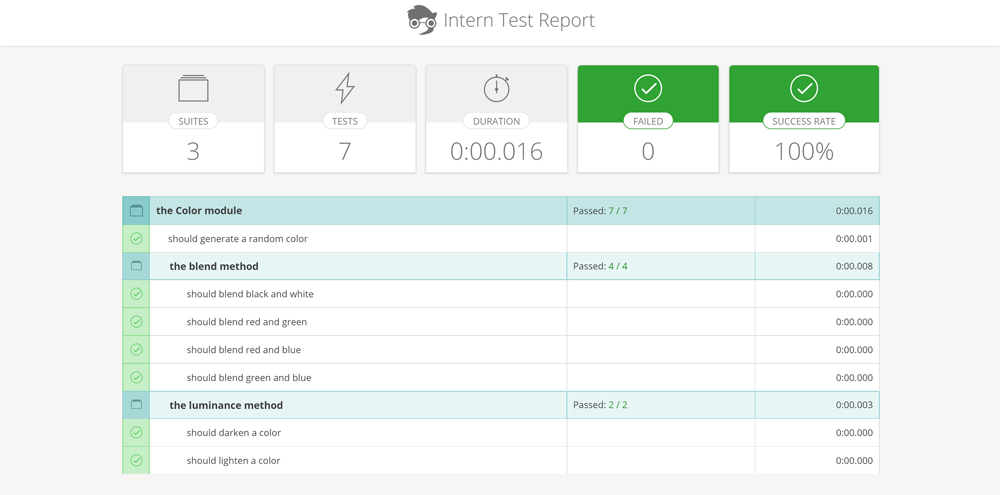
\includegraphics[width=\textwidth]{images/testing/intern}}
    \caption[Intern]{Intern user interface.}
    \label{fig:intern}
\end{figure}


		\emph{Jasmine} is often recommended and regarded as the most popular JS unit testing framework~\footnote{\bibentry{feldman2014testing}}. It has a simple setup, built-in assertions, is well supported, can adapt to other assertion libraries and performs code coverage when used with Istanbul. Jasmine also has an elegant, descriptive syntax that adheres to the BDD paradigm. However, its asynchronous testing support could be improved greatly, which is problematic for this particular project because asynchronous loading is used extensively.

		\emph{Mocha} proved to have a very simple setup, is highly extensible, very flexible, has good reporting and a BDD syntax that resembles Jasmine. It allows the use of any assertion library, enabling users to choose their preferred BDD style and offers great asynchronous testing and promise support. Mocha can also be integrated easily with Blanket, a code coverage tool. One issue with Mocha is that it has an overly simple and plain user interface, sometimes making it difficult to determine which tests have passed or failed.

		\emph{QUnit} was immediately discarded since it does not support the BDD paradigm, and instead utilises TDD.

		From these testing frameworks, \emph{Mocha} was chosen simply because of its fantastic asynchronous testing support and flexibility in choosing an assertion library and BDD style. Its user interface was transformed using customised CSS, which has been demonstrated in Figure~\ref{fig:mocha}, so the tests become more readable.

		\newcommand{\mochawidth}{0.496\textwidth}
\newcommand{\mochaheight}{4cm}
\begin{figure}[H]
	\centering
	\begin{subfigure}[b]{\mochawidth}
        \figureborder{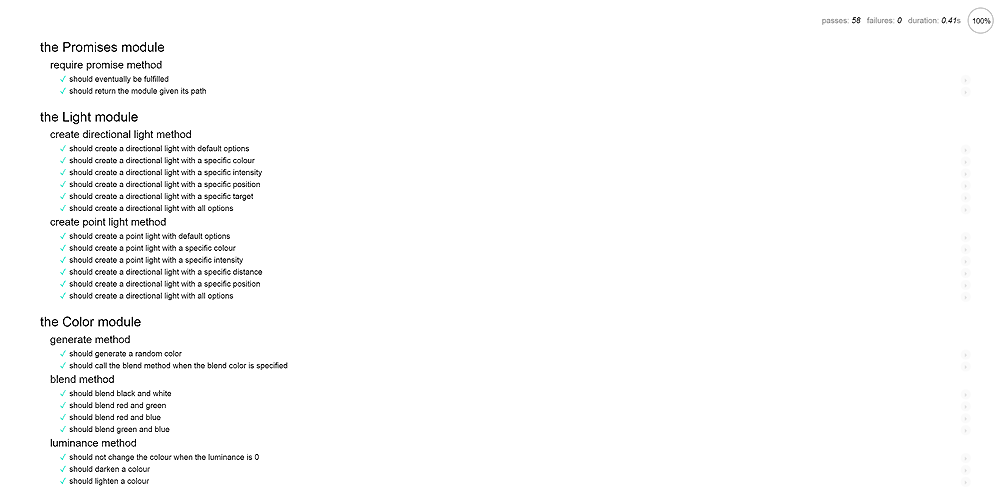
\includegraphics[width=\textwidth,height=\mochaheight]{images/testing/mocha_before}}
        \caption{Default Mocha interface.}
        \label{fig:mocha_before}
    \end{subfigure}
    \begin{subfigure}[b]{\mochawidth}
        \figureborder{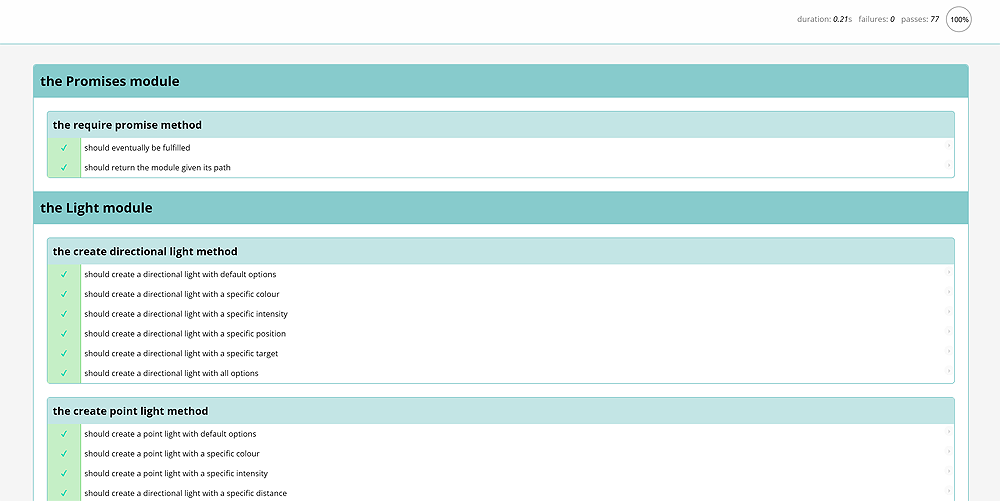
\includegraphics[width=\textwidth,height=\mochaheight]{images/testing/mocha_after}}
        \caption{Mocha interface after custom styling}
        \label{fig:mocha_after}
    \end{subfigure}
	\caption[Mocha]{Mocha styling}
	\label{fig:mocha}
\end{figure}


	}

}

\section{Assertions} {
\label{sec:assertions}

	\emph{Chai} assertions were used with the Mocha testing framework, as they offer great flexibility. Users are able to choose their preferred BDD style, which has been illustrated in Figure~\ref{fig:chai_assertions}.

	\newcommand{\assertionwidth}{0.328\textwidth}
\newcommand{\assertionsize}{\tiny}
\begin{figure}[H]
	\centering
	\begin{subfigure}[b]{\assertionwidth}
        \begin{lstlisting}[basicstyle=\assertionsize]
			chai.should();

			foo.should.be.a('string');
			foo.should.equal('bar');
			foo.should.have.length(3);
		\end{lstlisting}
        \caption{Should style}
        \label{fig:should_style}
    \end{subfigure}
    \begin{subfigure}[b]{\assertionwidth}
		\begin{lstlisting}[basicstyle=\assertionsize]
			var expect = chai.expect;
				
			expect(foo).to.be.a('string');
			expect(foo).to.equal('bar');
			expect(foo).to.have.length(3);
		\end{lstlisting}
        \caption{Expect style}
        \label{fig:expect_style}
    \end{subfigure}
    \begin{subfigure}[b]{\assertionwidth}
		\begin{lstlisting}[basicstyle=\assertionsize]
        var assert = chai.assert;

		assert.typeOf(foo, 'string');
		assert.equal(foo, 'bar');
		assert.lengthOf(foo, 3)
		\end{lstlisting}
        \caption{Assert style}
        \label{fig:assert_style}
    \end{subfigure}
	\caption[Chai assertions]{Chai assertion styles.}
	\label{fig:chai_assertions}
\end{figure}


	The \emph{should} style adheres to BDD and its behavioural specifications. However, this style extends \texttt{Object.prototype} which is generally considered bad practice. This style is not compatible in all browsers and results in scenarios where a test can fail~\footnote{\bibentry{luer2015assertion}}. Instead, the \emph{expect} style was used because it is compatible across all browsers and utilises chainable, natural language assertions. This style closely resembles BDD specifications, unlike the \emph{assert} style.

	\subsection{Asynchronous support} {
	\label{sec:testing_asynchronous_support}

		Mocha provides a way to test asynchronous code through the \texttt{done} callback or by returning a \texttt{Promise}~\footnote{\bibentry{holowaychuk2011mocha}}, which has been presented in Figure~\ref{fig:mocha_asynchronous_code}. Promises are used extensively when loading shaders, so it was important to have a clean way of testing asynchronous code. 

		\newcommand{\mochasize}{\scriptsize}
\begin{figure}[H]
	\centering
	\begin{subfigure}[b]{0.45\textwidth}
        \begin{lstlisting}[basicstyle=\mochasize]
			doSomethingAsync()
				.then(function (result) {
        			result.should.equal('foo');
        			done();
    			}
			);
		\end{lstlisting}
        \caption{Callback}
        \label{fig:mocha_callback}
    \end{subfigure}
    \begin{subfigure}[b]{0.5\textwidth}
		\begin{lstlisting}[basicstyle=\mochasize]
			return doSomethingAsync()
				.then(function (result) {
					// Return the result from the promise.
        			return result.should.equal('foo');
    			}
			);
		\end{lstlisting}
        \caption{Promise}
        \label{fig:mocha_promise}
    \end{subfigure}
	\caption[Mocha asynchronous code]{Mocha asynchronous code.}
	\label{fig:mocha_asynchronous_code}
\end{figure}


		However, this method of testing asynchronous code could be improved by using the \emph{Chai as Promised} plugin for Chai. This plugin extends Chai with a fluent language for asserting facts about promises~\footnote{\bibentry{denicola2012chaiaspromised}}. An example of this improvement has been illustrated in Figure~\ref{fig:chai_as_promised}, which transforms the assertion seen in Figure~\ref{fig:mocha_asynchronous_code} down to one line.

		%!TEX root = ../../../report.tex

\begin{figure}[H]
	\centering
	\begin{lstlisting}
		return doSomethingAsync().should.eventually.equal('foo');
	\end{lstlisting}
	\caption[Chai as Promised]{Chai as Promised.}
    \label{fig:chai_as_promised}
\end{figure}


	}

	\subsection{Spies, stubs and mocks} {
	\label{sec:testing_spy_stub_mock_support}

		Mocha is not equipped with spies, stubs or mocks~\footnote{\bibentry{holowaychuk2011mocha}} and instead recommend using \emph{Sinon.JS}, a popular library designed for this purpose. Similarly to Section~\ref{sec:testing_asynchronous_support}, a plugin called \emph{Sinon-Chai} provides a set of custom assertions for using the Sinon.JS spy, stub, and mocking framework with the Chai assertion library~\footnote{\bibentry{denicola2012sinonchai}}.

	}

}

\section{General structure} {
\label{sec:testing_structure}

	In Mocha, the \texttt{describe} keyword is a way to group tests together, while each \texttt{it} clause represents a single test case. A simple example of a test suite has been shown in Figure~\ref{fig:mocha_example}.

	%!TEX root = ../report.tex

\begin{figure}[H]
	\centering
    \begin{lstlisting}
		describe('Array', function() {
			describe('#indexOf()', function() {
				it('should return -1 when the value is not present', function() {
  					expect([1,2,3].indexOf(5)).to.equal(-1);
	    		});
			});
		});
	\end{lstlisting}
    \caption[Mocha]{Mocha example.}
    \label{fig:mocha_example}
\end{figure}


}

\section{Hooks} {
\label{sec:testing_hooks}

	Mocha provides \texttt{before}, \texttt{after}, \texttt{beforeEach} and \texttt{afterEach} hooks, which are described in Figure~\ref{fig:mocha_hooks}. These hooks can be used to set up preconditions or to perform test clean up~\footnote{\bibentry{holowaychuk2011mocha}}.

	\begin{figure}[H]
	\centering
	\begin{lstlisting}
		describe('hooks', function () {

			before(function () {
				// runs before all tests in this block
			});

			after(function () {
				// runs after all tests in this block
			});

			beforeEach(function () {
				// runs before each test in this block
			});

			afterEach(function () {
				// runs after each test in this block
			});

			// test cases

		});
	\end{lstlisting}
	\caption[Mocha hooks]{Mocha hooks.}
	\label{fig:mocha_hooks}
\end{figure}


	Typically, \texttt{beforeEach} and \texttt{afterEach} hooks were used when running tests to:

	\begin{itemize}
		\item Initialize shared variables.
		\item Create spies or stubs for methods that were called in each test suite.
		\item Perform common assertions after initialising a test case.
		\item Reset stubs or other data.
	\end{itemize}

}

\section{Style} {
\label{sec:testing_style}

	The style used throughout the Mocha documentation resembles Figure~\ref{fig:mocha_example} where the following is true:

	\begin{itemize}
		\item The top level \texttt{describe} represents the class name.
		\item Any proceeding \texttt{describe} clauses represent the method name in the form of \texttt{\#methodName()}.
		\item Each sentence in a test case may or may not be preceeded by \emph{should}.
	\end{itemize}

	This style was therefore found to be quite inconsistent and does not output the results in a human-readable format. Instead, the following style was developed and used when developing tests:

	\begin{itemize}
		\item The top level \texttt{describe} represents the name of the AMD module and reads as \texttt{the ModuleName module}.
			\begin{itemize}
				\item Preceeding the module name with the word \texttt{the} adheres the behavioural specifications by following a fluid sentence structure.
			\end{itemize}
		\item Any proceeding \texttt{describe} clauses represent the method name in the form of \texttt{methodName method}.
			\begin{itemize}
				\item Adding \texttt{method} to the end of each title makes the test case more human-readable.
			\end{itemize}
		\item Each sentence in a test case is preceeded by \emph{should}.
	\end{itemize}

	An example of this style has been demonstrated in Figure~\ref{fig:testing_style}.

	\begin{figure}[H]
	\centering
	\begin{lstlisting}
		describe('the Array module', function() {
			describe('indexOf method', function() {
				it('should return -1 when the value is not present', function() {
					expect([1,2,3].indexOf(5)).to.equal(-1);
				});
			});
		});
	\end{lstlisting}
	\caption[Testing style]{Testing style.}
	\label{fig:testing_style}
\end{figure}


}

\section{Example} {
\label{sec:testing_examples}

	%!TEX root = ../../../report.tex

\begin{figure}[H]
	\centering
	%!TEX root = ../../../report.tex

\begin{figure}[H]
	\centering
	\input{code/testing/mocha/example}
	\caption[Mocha example]{Mocha example.}
	\label{fig:mocha_example}
\end{figure}

	\caption[Mocha example]{Mocha example.}
	\label{fig:mocha_example}
\end{figure}


}

\section{Code coverage} {
\label{sec:code_coverage}

	Code coverage is the measurement of how many lines of code are executed while automated tests are running, making it a useful tool for finding untested code. Take the following snippet of code as an example:

	%!TEX root = ../../report.tex

\begin{lstlisting}
	if (condition) {
		// True condition - first branch
	} else {
		// False condition - second branch
	}
\end{lstlisting}


	If the \texttt{condition} is always \texttt{true}, then the second branch will never execute. Therefore, the unit test does not cover the false branch and this will be displayed in the results of a code coverage. Tests would ideally cover \textgreater80\% for a single test suite.

	\href{http://blanketjs.org/}{Blanket.js} was used in this project as a code coverage tool because it seamlessly integrates with Jasmine, Mocha and QUnit. Blanket injects the code coverage results at the bottom of the HTML page, which has been demonstrated in Figure~\ref{fig:blanket}.

	\begin{figure}[H]
	\centering
    \figureborder{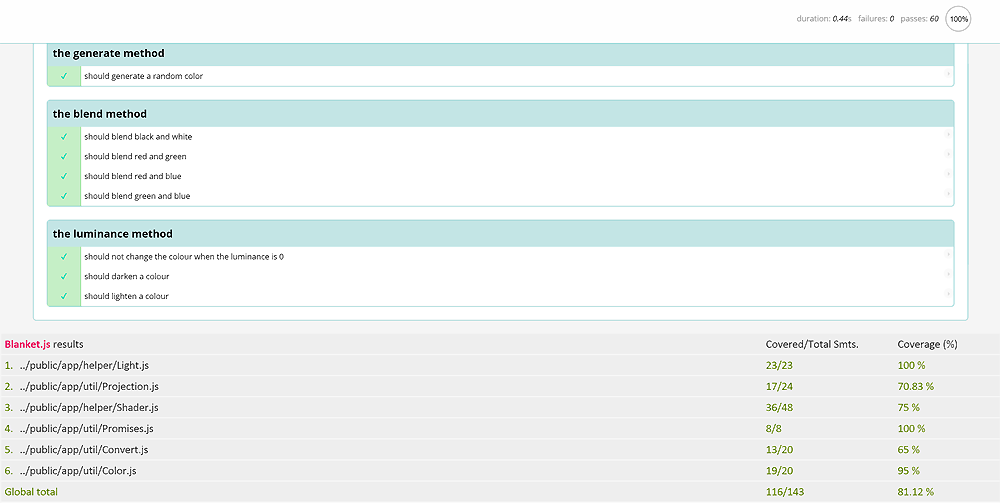
\includegraphics[width=\textwidth]{images/testing/blanket}}
    \caption[Blanket]{Blanket code coverage.}
    \label{fig:blanket}
\end{figure}


	A result from the code coverage can be expanded to reveal more information. It displays the entire file, including line numbers, and highlights the lines of code that were not covered under the tests that were executed. This behaviour can be identified in Figure~\ref{fig:code_coverage}, which demonstrates a method that was not tested.

	%!TEX root = ../../report.tex

\begin{lstlisting}
	if (condition) {
		// True condition - first branch
	} else {
		// False condition - second branch
	}
\end{lstlisting}


	Code coverage was evaluated after the creation of each test suite. When a test suite was analysed, more tests would be written in an attempt to improve the overall code coverage. This process was repeated until an acceptable amount of code coverage was reached.

}

\section{Performance testing} {
\label{sec:performance_testing}

	\todo{Introduce setup - selenium}

}

	}

	\todo{testing - results}

	\chapter{Results} {
	\label{ch:results}
		\begin{figure}[H]
	\centering
    \figureborder{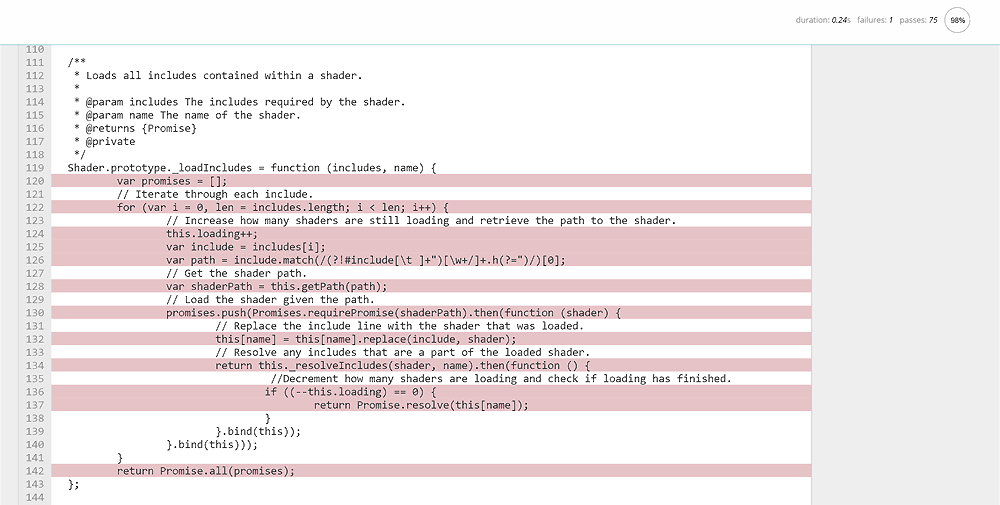
\includegraphics[width=\textwidth]{images/testing/coverage_results}}
    \caption[Code coverage results]{Code coverage results.}
    \label{fig:code_coverage_results}
\end{figure}

	}

	\todo{res - conc}

	\chapter{Conclusion} {
	\label{ch:conclusion}
		%!TEX root = ../report.tex

Conclusion.

overall usability of the system could be improved, especially by providing a small tutorial when opening the system and help tooltips.

future work = improve usability and performance of visualisations by moving processing to node.js and adding production scripts to decrease load time. consider merging geometries and removing some features in favour of performance.
	}
	
	\renewcommand{\bibname}{References}
	\printbibliography[notcategory=exclude]

	%!TEX root = report.tex

\appendix
\chapter{Architecture} {
\label{app:architecture}
	%!TEX root = ../../report.tex

\begin{figure}[H]
	\centering
    \includegraphics[width=\textwidth]{images/design/class_diagram}
    \caption[Class diagram]{The system architecture shown as a class diagram.}
    \label{fig:class_diagram}
\end{figure}

}

\chapter{System Usability Scale} {
\label{app:system_usability_scale}

	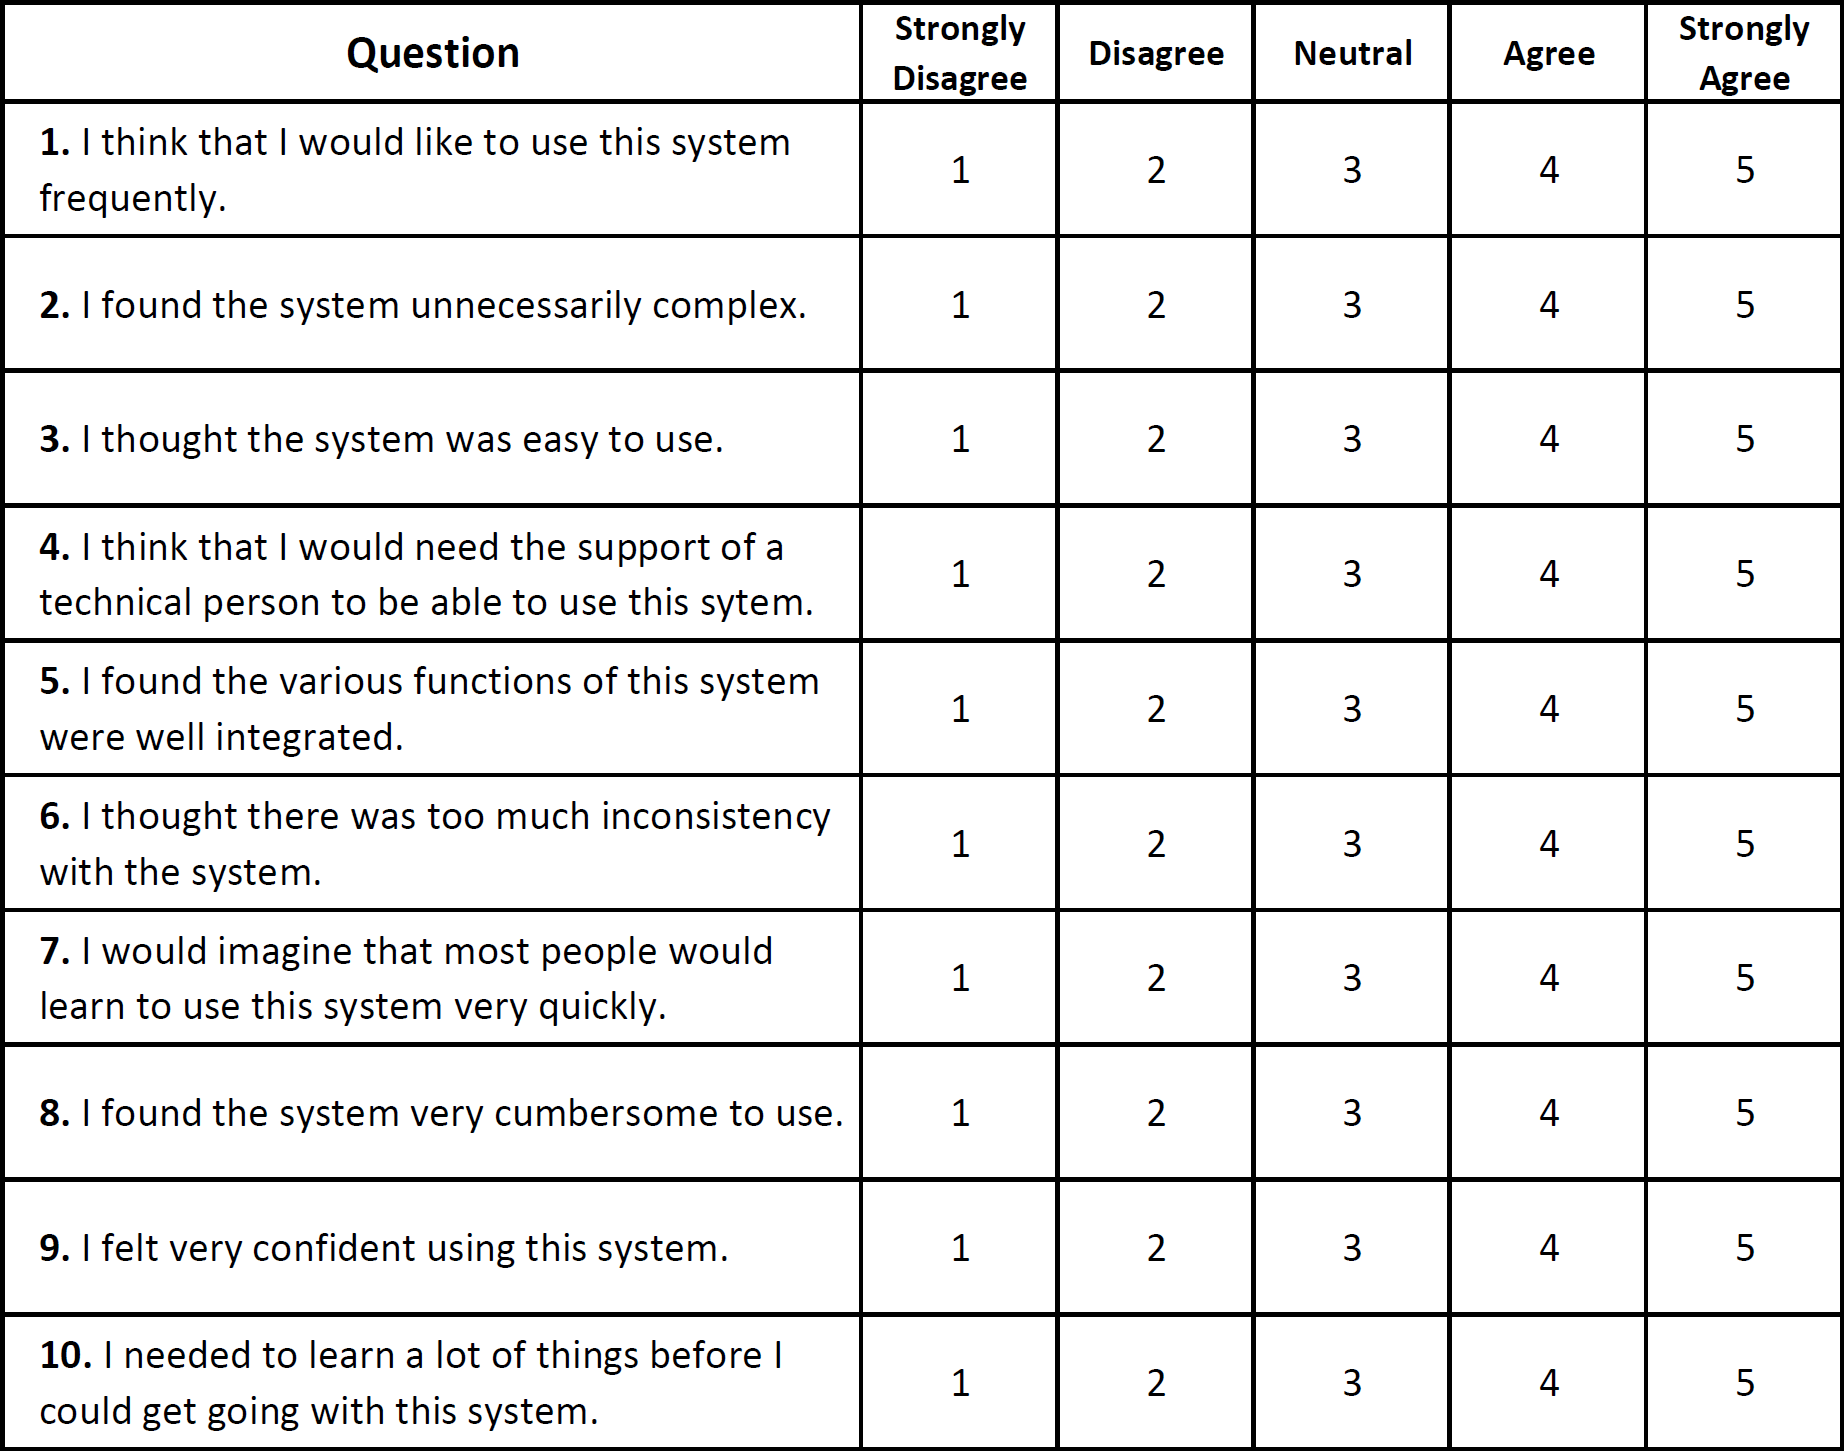
\includegraphics[width=\textwidth]{images/design/sus}

	The System Usability Scale (SUS) score is calculated by first converting each participant's score for each question to a new value. The values are obtained by performing $value - 1$ for each odd question and $5 - value$ for each even question. These values for each participant are then added together and multiplied by 2.5 to convert the original score from 0-40 to 0-100. Further, the SUS score should be considered in terms of percentile ranking instead of percentages.

	% \section{Questionnaire} {
	% \label{sec:questionnaire}

	% 	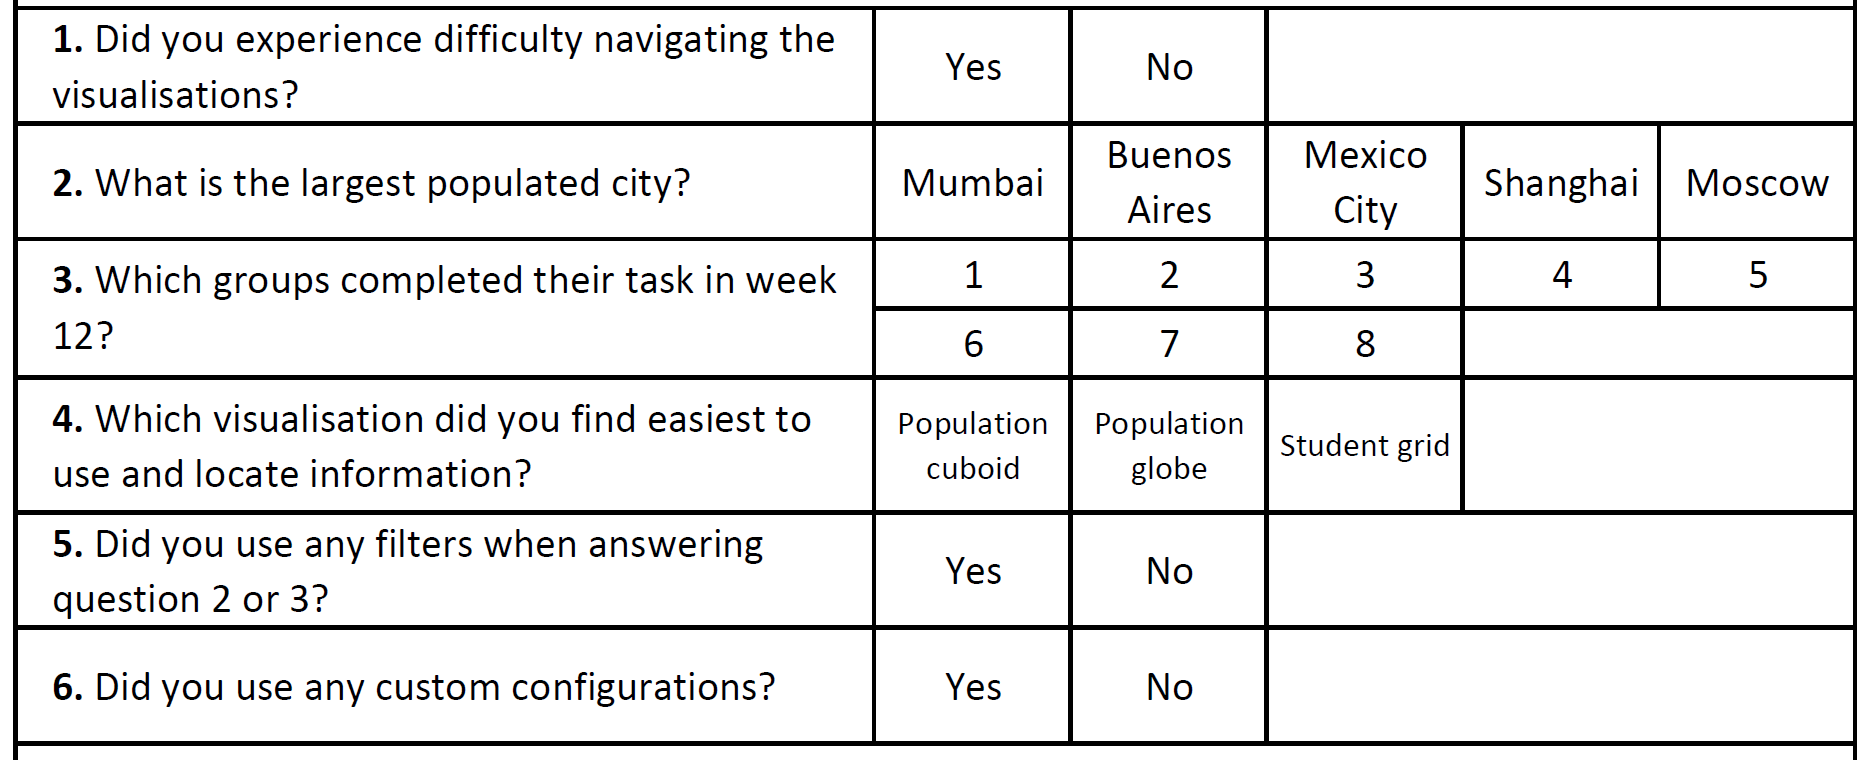
\includegraphics[width=\textwidth]{images/design/questionnaire}

	% }

}

\chapter{Testing} {

	\section{Mocha asynchronous support} {
	\label{app:mocha_asynchronous_support}
		%!TEX root = ../../../report.tex

\begin{figure}[H]
	\newcommand{\basicstyle}{\scriptsize}
    \captionsetup[subfigure]{aboveskip=0em,belowskip=-0.2em}
	\begin{subfigure}[b]{0.45\textwidth}
        %!TEX root = ../../../report.tex

\begin{lstlisting}[basicstyle=\basicstyle]
	doSomethingAsync()
		.then(function (result) {
			result.should.equal('foo');
			done();
		}
	);
\end{lstlisting}

        \caption{Callback}
        \label{fig:mocha_callback}
    \end{subfigure}
    \begin{subfigure}[b]{0.55\textwidth}
		%!TEX root = ../../../report.tex

\begin{lstlisting}[basicstyle=\basicstyle]
	return doSomethingAsync()
		.then(function (result) {
			// Return the result from the promise.
			return result.should.equal('foo');
		}
	);
\end{lstlisting}

        \caption{Promise}
        \label{fig:mocha_promise}
    \end{subfigure}
	\caption{Mocha asynchronous support.}
	\label{fig:mocha_asynchronous_support}
\end{figure}

	}

	\section{Chai as Promised} {
	\label{app:chai_as_promised}
		%!TEX root = ../../../report.tex

\begin{figure}[H]
	\centering
	\begin{lstlisting}
		return doSomethingAsync().should.eventually.equal('foo');
	\end{lstlisting}
	\caption[Chai as Promised]{Chai as Promised.}
    \label{fig:chai_as_promised}
\end{figure}

	}

	\section{Mocha structure} {
	\label{app:mocha_structure}
		%!TEX root = ../../../report.tex

\begin{lstlisting}
	describe('Array', function() {
		describe('#indexOf()', function() {
			it('should return -1 when the value is not present', function() {
				expect([1,2,3].indexOf(5)).to.equal(-1);
			});
		});
	});
\end{lstlisting}

	}

	\section{Mocha hooks} {
	\label{app:mocha_hooks}
		\begin{figure}[H]
	\centering
	\begin{lstlisting}
		describe('hooks', function () {

			before(function () {
				// runs before all tests in this block
			});

			after(function () {
				// runs after all tests in this block
			});

			beforeEach(function () {
				// runs before each test in this block
			});

			afterEach(function () {
				// runs after each test in this block
			});

			// test cases

		});
	\end{lstlisting}
	\caption[Mocha hooks]{Mocha hooks.}
	\label{fig:mocha_hooks}
\end{figure}

	}

	\section{Testing style} {
	\label{app:testing_style}
		%!TEX root = ../../report.tex

\begin{figure}[H]
	\centering
	%!TEX root = ../../report.tex

\begin{figure}[H]
	\centering
	\input{code/testing/style}
	\caption[Testing style]{Testing style.}
	\label{fig:testing_style}
\end{figure}

	\caption[Testing style]{Testing style.}
	\label{fig:testing_style}
\end{figure}

	}
	
}
	
\end{document}
